\documentclass[acmsmall,screen,nonacm]{acmart}

\citestyle{acmauthoryear}
\usepackage{xr}
\externaldocument[M-]{../ghb}
% Generated by simulations/make_numbers.py. Do not edit.
\newcommand{\SimOneChecks}{101}
\newcommand{\SimOneWithin}{98\%}
\newcommand{\SimOneMaxRel}{1.6\%}
\newcommand{\SimOneReps}{40{,}000}
\newcommand{\SimTwoWorstGHB}{1.02}
\newcommand{\SimTwoWorstPool}{382}
\newcommand{\SimTwoMeanPool}{134}
\newcommand{\SimTwoMinGHB}{0.12}
\newcommand{\SimTwoMinOracle}{0.07}
\newcommand{\SimThreeB}{46}
\newcommand{\SimThreeSmall}{2.28}
\newcommand{\SimThreeLarge}{1.08}
\newcommand{\SimThreeMin}{1.05}
\newcommand{\SimThreePoolSmall}{1.44}
\newcommand{\SimThreePoolLarge}{0.15}
\newcommand{\SimThreeKThreeOracle}{0.78}
\newcommand{\SimThreeKThreeDL}{0.91}
\newcommand{\SimThreeKThreeBayes}{0.93}
\newcommand{\SimThreeKFortyEightDL}{0.68}
\newcommand{\SimThreeKFortyEightOracle}{0.66}
\newcommand{\SimFourRingLam}{0.977}
\newcommand{\SimFourRingPred}{203}
\newcommand{\SimFourRingTwo}{35}
\newcommand{\SimFourRegionalLam}{0.964}
\newcommand{\SimFourRegionalPred}{127}
\newcommand{\SimFourRegionalTwo}{22}
\newcommand{\SimFourRandomLam}{0.937}
\newcommand{\SimFourRandomPred}{73}
\newcommand{\SimFourRandomTwo}{11}
\newcommand{\SimFourTwohopLam}{0.933}
\newcommand{\SimFourTwohopPred}{69}
\newcommand{\SimFourTwohopTwo}{14}
\newcommand{\SimFiveMixedGOneEpsTenth}{19.3}
\newcommand{\SimFiveMixedGOneEpsOne}{43.7}
\newcommand{\SimFiveMixedGEightEpsTenth}{21.0}
\newcommand{\SimFiveMixedGEightEpsOne}{45.0}
\newcommand{\SimFiveSmallGOneEpsTenth}{1.0}
\newcommand{\SimFiveSmallGOneEpsOne}{30.6}
\newcommand{\SimFiveSmallGEightEpsTenth}{6.9}
\newcommand{\SimFiveSmallGEightEpsOne}{41.4}
\newcommand{\SimSixGHBLow}{0.31}
\newcommand{\SimSixGMRFLow}{0.40}
\newcommand{\SimSixGHBHigh}{0.94}
\newcommand{\SimSixGMRFHigh}{0.40}
\newcommand{\SimSixBeta}{46}
\newcommand{\SimSevenLocal}{0.0266}
\newcommand{\SimSevenGHB}{0.0182}
\newcommand{\SimSevenGlobal}{0.0173}
\newcommand{\SimSevenReduction}{31\%}
\newcommand{\SimSevenGHBNoDP}{0.0110}
\newcommand{\SimSevenGHBTenth}{0.0285}
\newcommand{\SimSevenLocalTenth}{0.0273}
\newcommand{\SimSevenWorstRatio}{0.94}
\newcommand{\SimSevenGlobalWorstRatio}{2.48}

\graphicspath{{../../Collectively_Big_Locally_Small/supplement/}}
\renewcommand{\thesection}{S\arabic{section}}
\renewcommand{\thefigure}{S\arabic{figure}}
\renewcommand{\thetable}{S\arabic{table}}

\usepackage{tabularx}
\usepackage{enumitem}
\usepackage{makecell}
\usepackage{longtable}
\setlist[enumerate]{itemsep=2pt}
\usepackage{pifont}
\usepackage[ruled,vlined,linesnumbered]{algorithm2e}
\SetAlFnt{\small}
\usepackage{multirow}
\usepackage{tikz}
\usetikzlibrary{arrows.meta,positioning}

% Colours of the TikZ figures
\definecolor{edgec}{rgb}{0.3851,0.41255,0.44}
\definecolor{slate100}{rgb}{0.9451,0.96078,0.97647}
\definecolor{red100}{rgb}{0.99608,0.88628,0.88628}
\definecolor{teal100}{rgb}{0.8,0.98431,0.9451}
\definecolor{blue100}{rgb}{0.85883,0.91765,0.99608}
\definecolor{amber100}{rgb}{0.99608,0.95294,0.7804}
\definecolor{violet100}{rgb}{0.92941,0.91374,0.99608}
\definecolor{hdrc}{rgb}{0.12158,0.16078,0.2}
\definecolor{conc}{rgb}{0.47295,0.49648,0.52}
\definecolor{famO}{rgb}{0.7255,0.1098,0.1098}
\definecolor{famE}{rgb}{0.14511,0.38824,0.92157}
\definecolor{famT}{rgb}{0.85098,0.46667,0.02353}
\definecolor{famC}{rgb}{0.05882,0.46275,0.43137}
\definecolor{violetc}{rgb}{0.48627,0.22745,0.92941}
\definecolor{grayc}{rgb}{0.60393,0.64706,0.69412}
\definecolor{gray600}{rgb}{0.29727,0.32863,0.36}

\newcommand{\eff}{\mathrm{eff}}
\newcommand{\yes}{\textcolor{famC}{\ding{51}}}
\newcommand{\no}{\textcolor{famO}{\ding{55}}}
\newcommand{\partly}{\textcolor{famT}{$\boldsymbol{\circ}$}}

\AtEndPreamble{%
 \theoremstyle{acmdefinition}
 \newtheorem{remark}[theorem]{Remark}}

\begin{document}

\title{Borrowing Strength Without Borrowing Data: Online Supplement}
\subtitle{Simulation study, real hospital networks and the design of GHB}

\author{Sancho Amaral Sim\~{o}es}
\email{sanchosimoes@student.dei.uc.pt}
\affiliation{%
 \institution{CISUC, DEI, FCTUC, University of Coimbra}
 \city{Coimbra}
 \country{Portugal}}

\author{Jo\~{a}o P. Vilela}
\email{jvilela@fc.up.pt}
\affiliation{%
 \institution{CISUC, DEI, FCTUC, University of Coimbra}
 \city{Coimbra}
 \country{Portugal}}
\affiliation{%
 \institution{CRACS/INESC TEC, DCS, FCUP, University of Porto}
 \city{Porto}
 \country{Portugal}}

\author{Pedro Henriques Abreu}
\email{pha@dei.uc.pt}
\affiliation{%
 \institution{CISUC, DEI, FCTUC, University of Coimbra}
 \city{Coimbra}
 \country{Portugal}}

\begin{abstract}
This supplement accompanies the paper \emph{Borrowing Strength Without Borrowing Data: Private, Serverless and Tuning-Free Collaboration with Graph Hierarchical Borrowing}. Section~\ref{sec:sims} gives the full design and results of the eighteen simulations of Section~\ref{M-sec:experiments}. Section~\ref{sec:tcga} documents the TCGA study of Section~\ref{M-sec:real-tcga}: data, protocol, the configurations fixed for every literature method, the design results, the oracle arm, tuning GHB, and the design choices. Sections~\ref{sec:flamby} and~\ref{sec:images} document the FLamby benchmark and the image study, Section~\ref{sec:eight} every network's results for the small networks of Section~\ref{M-sec:real-eight}, and Section~\ref{sec:real} every hospital's results on UCI Heart Disease. Section~\ref{sec:revision} records how GHB-lite was designed and the extensions that were tried and not adopted. Numbers are generated by the released scripts and read into the text as LaTeX macros, except a few from development runs, whose scripts are named where they appear.
\end{abstract}

\maketitle
\renewcommand{\shortauthors}{Sim\~{o}es et al.}

%% ===================================================================
\section{Simulation Study}\label{sec:sims}

Section~\ref{M-sec:experiments} of the paper summarizes these simulations; this section gives the full design and every figure. The simulations test GHB-lite (Sections~\ref{M-sec:model} and~\ref{M-sec:heads} of the paper) under its own model and under a logistic analogue. They check internal consistency and expose the cost of estimating the unknown quantities that Propositions~\ref{M-prop:borrowing} to~\ref{M-prop:gossip} take as known; they are not evidence about real hospital networks. Unless stated otherwise, the network has 24 hospitals whose sizes are drawn once from a log-normal distribution with median 100 and clipped (16 to 479 patients), $\sigma^2=1$, $\delta=10^{-5}$, clipping bound $C=1$, and the privatized releases are averaged by 60 rounds of Metropolis-Hastings gossip on the ring with two-hop links of Figure~\ref{M-fig:gossip}. \emph{Plug-in GHB-lite} estimates everything it needs from the privatized releases and public quantities only: $\tau^2$ by DerSimonian-Laird \cite{dersimonian1986meta} (Remark~\ref{M-rem:tau}), the leave-one-out population estimate by inverse-variance weighting, and its error $M$ from those weights. Risk is reported relative to local estimation, $R_k/v_k$ with $v_k=\sigma^2/n_k$; values below 1 mean that a hospital gains. All code is in \texttt{simulations/} of the companion survey's repository, and \texttt{run\_all.py} regenerates every figure and number in about twenty minutes.

\paragraph{Simulation 1: the closed forms} Figure~\ref{fig:s1} and Tables~\ref{tab:s1} and~\ref{tab:s1M} repeat the setting of Figure~\ref{M-fig:risk} with \SimOneReps{} replicates per point. Across \SimOneChecks{} comparisons of a simulated risk or $M$ with its closed form, \SimOneWithin{} lie within two Monte Carlo standard errors, and the largest relative deviation is \SimOneMaxRel. Propositions~\ref{M-prop:borrowing} and~\ref{M-prop:privatized} and the code that draws Figure~\ref{M-fig:risk} agree.

\begin{figure}[t]
\centering
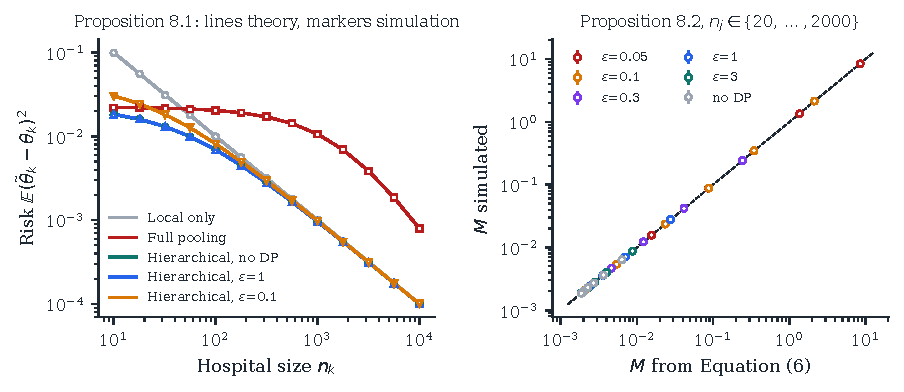
\includegraphics[width=\linewidth]{figures/s1_validate}
\caption{Simulation 1. Left: risk against hospital size; lines are the closed forms of Figure~\ref{M-fig:risk}, markers are simulated ($\pm 2$ standard errors). Right: simulated $M$ of the privatized leave-one-out mean against Equation~\eqref{M-eq:M}, for 11 other hospitals of 20 to 2,000 patients and six privacy budgets.}
\label{fig:s1}
\end{figure}

\begin{table}[t]
\caption{Simulation 1: exact values behind Figure~\ref{fig:s1}. Top: risk $R_k$ of a hospital of $n_k$ patients ($\sigma^2=1$), simulated, with the closed form in grey; Global: full pooling without privacy; Hier.: hierarchical borrowing with known $\tau^2$. Bottom: simulated $M$ of the privatized leave-one-out mean, when the 11 other hospitals all have $n_j$ patients, with Equation~\eqref{M-eq:M} in grey.}
\label{tab:s1}
\scriptsize
\setlength{\tabcolsep}{4pt}
\begin{tabular}{@{}rlllll@{}}
\toprule
$n_k$ & Local & Global & Hier., no DP & Hier., $\epsilon=1$ & Hier., $\epsilon=0.1$\\
\midrule
\csname @@input\endcsname../../Collectively_Big_Locally_Small/supplement/results/tables/s_sim1_risk.tex 
\bottomrule
\end{tabular}
\end{table}

\begin{table}[t]
\caption{Simulation 1, continued: $M$ against the size $n_j$ of the other hospitals and the privacy budget; simulated, with Equation~\eqref{M-eq:M} in grey.}
\label{tab:s1M}
\scriptsize
\setlength{\tabcolsep}{4pt}
\begin{tabular}{@{}rllllll@{}}
\toprule
$n_j$ & $\epsilon=0.05$ & $\epsilon=0.1$ & $\epsilon=0.3$ & $\epsilon=1$ & $\epsilon=3$ & no DP\\
\midrule
\csname @@input\endcsname../../Collectively_Big_Locally_Small/supplement/results/tables/s_sim1_M.tex 
\bottomrule
\end{tabular}
\end{table}


\paragraph{Simulation 2: heterogeneity} Figure~\ref{fig:s2} and Table~\ref{tab:s2} vary $\tau^2$ from $10^{-4}$ to 1. Plug-in GHB-lite is never worse than local estimation by more than Monte Carlo error: its worst hospital reaches a relative risk of \SimTwoWorstGHB{} at most. A single global model (the sample-size weighted mean of all site estimates, computed without privacy) is the best choice when $\tau^2$ is tiny, but its mean relative risk reaches \SimTwoMeanPool{} and its worst hospital \SimTwoWorstPool{} at $\tau^2=1$. Estimating $\tau^2$ costs most when heterogeneity is smallest: at $\tau^2=10^{-4}$ and $\epsilon=1$ the plug-in reaches \SimTwoMinGHB{} against \SimTwoMinOracle{} with the true $\tau^2$. Gossip with 60 rounds is indistinguishable from exact averaging.

\begin{figure}[t]
\centering
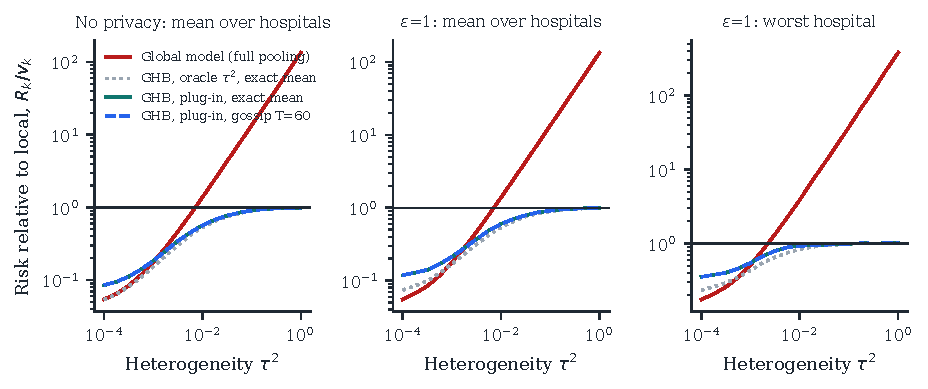
\includegraphics[width=\linewidth]{figures/s2_heterogeneity}
\caption{Simulation 2. Risk relative to local estimation as a function of heterogeneity, mean over hospitals without privacy and with $\epsilon=1$, and for the worst hospital with $\epsilon=1$.}
\label{fig:s2}
\end{figure}

\begin{table}[t]
\caption{Simulation 2: exact values behind Figure~\ref{fig:s2}. Relative risk $R_k/v_k$, mean over hospitals and worst hospital, at $\epsilon=1$ (top) and without privacy (bottom). Global: full pooling, without privacy in both blocks; Oracle: GHB-lite with the true $\tau^2$ and exact averaging; Plug-in: DerSimonian-Laird \cite{dersimonian1986meta}, with exact averaging or 60 gossip rounds; FB: $\tau$ integrated out (Remark~\ref{M-rem:tau}), 60 gossip rounds.}
\label{tab:s2}
\scriptsize
\setlength{\tabcolsep}{3.5pt}
\begin{tabular}{@{}r*{10}{r}@{}}
\toprule
& \multicolumn{2}{c}{Global} & \multicolumn{2}{c}{Oracle} & \multicolumn{2}{c}{Plug-in, exact} & \multicolumn{2}{c}{Plug-in, gossip} & \multicolumn{2}{c}{FB, gossip}\\
\cmidrule(lr){2-3}\cmidrule(lr){4-5}\cmidrule(lr){6-7}\cmidrule(lr){8-9}\cmidrule(l){10-11}
$\tau^2$ & mean & worst & mean & worst & mean & worst & mean & worst & mean & worst\\
\midrule
\csname @@input\endcsname../../Collectively_Big_Locally_Small/supplement/results/tables/s_sim2_eps1.tex 
\midrule
\csname @@input\endcsname../../Collectively_Big_Locally_Small/supplement/results/tables/s_sim2_nodp.tex 
\bottomrule
\end{tabular}
\end{table}


\paragraph{Simulation 3: who gains, and how many hospitals are needed} At $\tau^2=0.02$ and $\epsilon=1$ (Figure~\ref{fig:s3}, left), every hospital gains about the same number of virtual patients, $B\approx\SimThreeB$, as Equation~\eqref{M-eq:borrowed} predicts. The hospitals with 60 patients or fewer multiply their effective sample size by \SimThreeSmall{} on average, and those with 300 or more by \SimThreeLarge{}; the smallest gain of any hospital is \SimThreeMin. The global model multiplies the effective sample size of small hospitals by \SimThreePoolSmall{} but cuts that of large hospitals to \SimThreePoolLarge{} of their own. With few hospitals, $\tau^2$ is poorly estimated (Figure~\ref{fig:s3}, right, and Table~\ref{tab:s3}). With three hospitals the mean relative risk is \SimThreeKThreeDL{} with DerSimonian-Laird \cite{dersimonian1986meta} against \SimThreeKThreeOracle{} with the true $\tau^2$, and the gap closes as the network grows (\SimThreeKFortyEightDL{} against \SimThreeKFortyEightOracle{} with 48 hospitals). The posterior mean of $\tau^2$ under a half-Cauchy(0.5) prior on $\tau$, the weakly informative choice that Remark~\ref{M-rem:tau} recommends, does better than DerSimonian-Laird \cite{dersimonian1986meta} from four hospitals upward but not with three.

\begin{figure}[t]
\centering
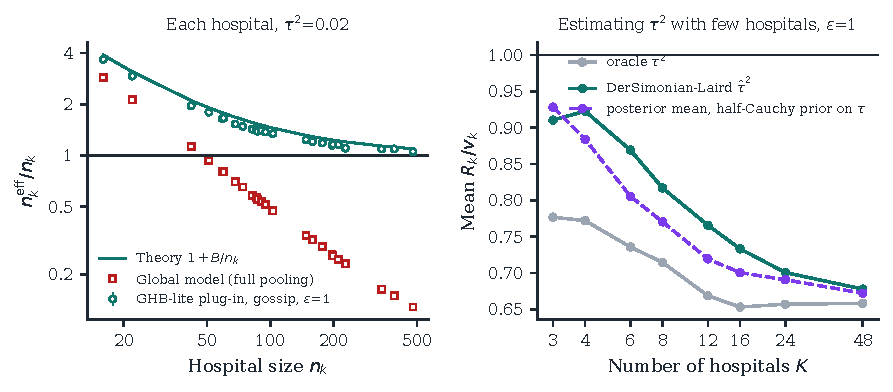
\includegraphics[width=\linewidth]{figures/s3_equity}
\caption{Simulation 3. Left: effective sample size relative to own size for each hospital, plug-in GHB-lite and a global model; the line is $1+B/n_k$. Right: mean relative risk against the number of hospitals for three ways of obtaining $\tau^2$.}
\label{fig:s3}
\end{figure}

\begin{table}[t]
\caption{Simulation 3: exact values behind Figure~\ref{fig:s3}, right. Mean relative risk against the number of hospitals $K$, for the true $\tau^2$, DerSimonian-Laird \cite{dersimonian1986meta}, and the posterior mean under a half-Cauchy(0.5) prior on $\tau$.}
\label{tab:s3}
\footnotesize
\begin{tabular}{@{}rrrr@{}}
\toprule
$K$ & True $\tau^2$ & DerSimonian-Laird \cite{dersimonian1986meta} & Posterior mean\\
\midrule
\csname @@input\endcsname../../Collectively_Big_Locally_Small/supplement/results/tables/s_sim3.tex 
\bottomrule
\end{tabular}
\end{table}


\paragraph{Simulation 4: gossip rounds} Figure~\ref{fig:s4} and Table~\ref{tab:s4} show the mean relative risk of plug-in GHB-lite after $T$ rounds of gossip on the four topologies of Figure~\ref{M-fig:gossip}. The risk comes within 2\% of its exact-average value after \SimFourRingTwo{} rounds on the ring, \SimFourRegionalTwo{} on the regional clusters, \SimFourRandomTwo{} on the sparse random graph and \SimFourTwohopTwo{} on the ring with two-hop links, far fewer than the rounds that the worst-case bound of Proposition~\ref{M-prop:gossip} requires for a consensus error of 1\% (\SimFourRingPred, \SimFourRegionalPred, \SimFourRandomPred{} and \SimFourTwohopPred). The bound is conservative for the risk: it controls the consensus error of the releases, while the risk depends on that error only through a population estimate that the shrinkage weight already discounts. After a single round on the ring, GHB-lite is worse than local estimation (relative risk 1.13), so a hospital should not use the borrowed estimate before the gossip has mixed.

\begin{figure}[t]
\centering
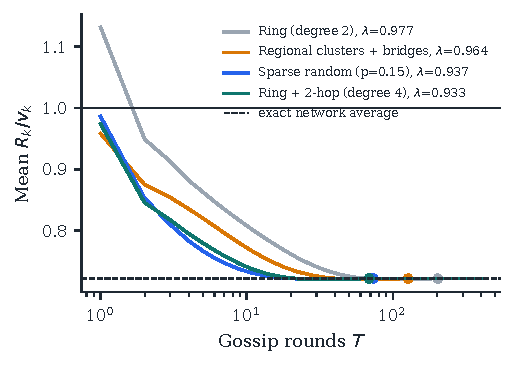
\includegraphics[width=0.62\linewidth]{figures/s4_gossip}
\caption{Simulation 4. Mean relative risk of plug-in GHB-lite against the number of gossip rounds ($\tau^2=0.02$, $\epsilon=1$). Dots mark $\log(100)/(1-\lambda)$; the dashed line is the exact network average.}
\label{fig:s4}
\end{figure}

\begin{table}[t]
\caption{Simulation 4: exact values behind Figure~\ref{fig:s4}. Mean relative risk of plug-in GHB-lite after $T$ gossip rounds on each topology; below, the second-largest eigenvalue modulus $\lambda$ of the gossip matrix, the rounds after which the risk is within 2\% of exact averaging, and the rounds that Proposition~\ref{M-prop:gossip} requires for a consensus error of 1\%.}
\label{tab:s4}
\scriptsize
\begin{tabular}{@{}lrrrr@{}}
\toprule
$T$ & Ring & Regional & Sparse random & Ring + 2-hop\\
\midrule
\csname @@input\endcsname../../Collectively_Big_Locally_Small/supplement/results/tables/s_sim4.tex 
\bottomrule
\end{tabular}
\end{table}


\paragraph{Simulation 5: joint release by small hospitals} Section~\ref{M-sec:privacy} proposes that small hospitals release jointly through secure aggregation, so that the privacy noise is calibrated to the group. Figure~\ref{fig:s5} and Table~\ref{tab:s5} show that the remedy matters only when every hospital is small. In a network of 16 hospitals of 20 patients and 8 of 200, the large hospitals dominate the inverse-variance weighted population estimate, and groups of eight raise the borrowed patients only from \SimFiveMixedGOneEpsTenth{} to \SimFiveMixedGEightEpsTenth{} at $\epsilon=0.1$. In a network of 24 hospitals of 20 patients, the same grouping raises $B$ from \SimFiveSmallGOneEpsTenth{} to \SimFiveSmallGEightEpsTenth{} at $\epsilon=0.1$ and from \SimFiveSmallGOneEpsOne{} to \SimFiveSmallGEightEpsOne{} at $\epsilon=1$.

\begin{figure}[t]
\centering
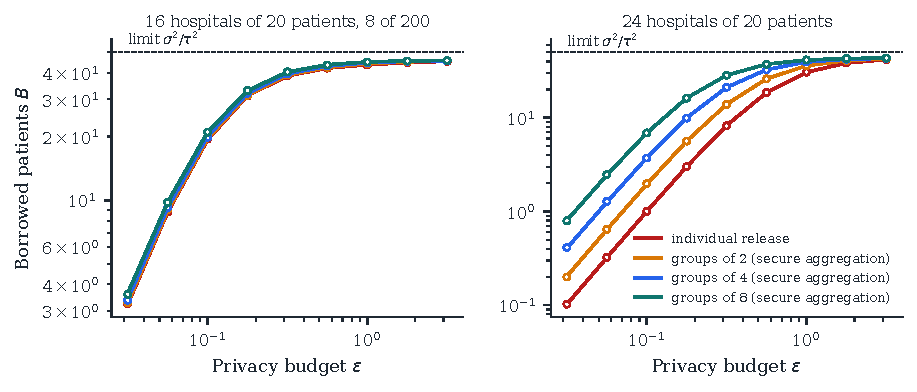
\includegraphics[width=\linewidth]{figures/s5_joint_release}
\caption{Simulation 5. Borrowed patients $B$ against the privacy budget for individual and joint release; lines are closed forms, markers simulation.}
\label{fig:s5}
\end{figure}

\begin{table}[t]
\caption{Simulation 5: exact values behind Figure~\ref{fig:s5}. Borrowed patients $B$ for groups of $g$ hospitals releasing jointly, simulated, with the closed form in parentheses. All small: 24 hospitals of 20 patients; mixed: 16 of 20 and 8 of 200 ($\tau^2=0.02$).}
\label{tab:s5}
\scriptsize
\begin{tabular}{@{}lrrrrr@{}}
\toprule
Network & $\epsilon$ & $g=1$ & $g=2$ & $g=4$ & $g=8$\\
\midrule
\csname @@input\endcsname../../Collectively_Big_Locally_Small/supplement/results/tables/s_sim5.tex 
\bottomrule
\end{tabular}
\end{table}


\paragraph{Simulation 6: structured heterogeneity} The 24 hospitals are split into four regions of six; $\theta_k$ is the sum of a regional effect with variance $\tau_r^2$ and a hospital effect with variance $\tau_w^2=0.002$. The GMRF prior of Equation~\eqref{M-eq:gmrf} links hospitals of the same region and is computed by Jacobi iterations on the privatized releases, followed by each hospital's local update with its own noise-free estimate. Its anchor term is switched off so that it uses the same information as the exchangeable prior, and its smoothing weight $\beta$ was chosen on separate tuning replicates (the same value, $\beta\approx\SimSixBeta$, was selected at every $\tau_r^2$); the regions are assumed known. Figure~\ref{fig:s6} and Table~\ref{tab:s6} show a crossover. When regions barely differ ($\tau_r^2\lesssim 0.003$), the exchangeable prior is better (\SimSixGHBLow{} against \SimSixGMRFLow{} at the smallest $\tau_r^2$), because the GMRF borrows only from five neighbors. When regional differences dominate, the exchangeable prior loses its gain (\SimSixGHBHigh) while the GMRF keeps it (\SimSixGMRFHigh).

\begin{figure}[t]
\centering
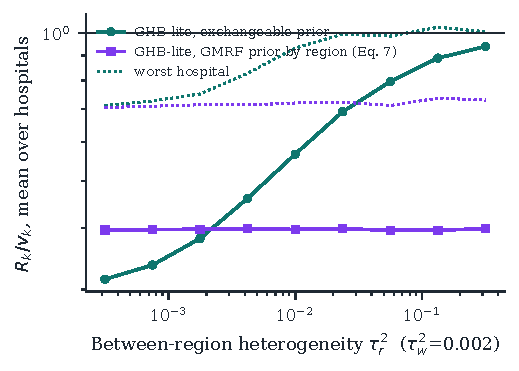
\includegraphics[width=0.62\linewidth]{figures/s6_gmrf}
\caption{Simulation 6. Mean relative risk (solid) and worst hospital (dotted) for the exchangeable and the regional GMRF prior, against the between-region variance ($\epsilon=1$).}
\label{fig:s6}
\end{figure}

\begin{table}[t]
\caption{Simulation 6: exact values behind Figure~\ref{fig:s6}. Mean and worst relative risk for the exchangeable prior and the regional GMRF prior against the between-region variance $\tau_r^2$ ($\epsilon=1$).}
\label{tab:s6}
\footnotesize
\begin{tabular}{@{}rrrrr@{}}
\toprule
& \multicolumn{2}{c}{Mean} & \multicolumn{2}{c}{Worst hospital}\\
\cmidrule(lr){2-3}\cmidrule(l){4-5}
$\tau_r^2$ & Exchangeable & GMRF & Exchangeable & GMRF\\
\midrule
\csname @@input\endcsname../../Collectively_Big_Locally_Small/supplement/results/tables/s_sim6.tex 
\bottomrule
\end{tabular}
\end{table}


\paragraph{Simulation 7: logistic-regression heads} This simulation leaves the Gaussian model. Each hospital has its own logistic model on four standardized features and an intercept, $\theta_k=\mu+u_k$ with $u_k\sim\mathcal{N}(0,\tau^2 I)$, and features are clipped so that $\|x\|\le\sqrt{5}$. Here $\mu_0$ is a published model (channel P3), equal to $\mu$ plus noise of standard deviation 0.3. Each hospital releases its mean score at $\mu_0$, $g_k=\frac{1}{n_k}\sum_i x_i(y_i-\sigma(x_i^\top\mu_0))$, plus isotropic Gaussian noise. Its $\ell_2$ sensitivity is $2\sqrt{5}/n_k$, and the noise is calibrated with zero-concentrated DP: $s_k=\Delta_k/\sqrt{2\rho}$ with $\rho+2\sqrt{\rho\ln(1/\delta)}=\epsilon$. Under the public feature distribution, $\mathbb{E}g_k=m(\theta_k)-m(\mu_0)$ with $m(\theta)=\mathbb{E}[x\,\sigma(x^\top\theta)]$, so the releases are mapped to the parameter scale by moment matching, linearized first at the pooled moment estimate and then at each hospital's leave-one-out network estimate; their variances follow by the delta method. The anchor shapes that second point only for hospitals where it passes the conflict check against the anchor-free network estimate. GHB-lite then borrows coordinatewise. Each hospital summarizes the posterior of $\tau$ (half-Cauchy(0.5) prior) by 12 quantiles, combines each component's network estimate with $\mu_0$ by precision weighting unless it dropped the anchor, multiplies by the weakly informative default $\mathcal{N}(0,2.5^2)$ \cite{gelman2008weakly}, and averages its maximum a posteriori fits under the components, weighted by the Laplace approximation of the marginal likelihood of its own data (Remark~\ref{M-rem:tau}). The code is \texttt{simulations/ghb\_logit.py}. The baselines are a local model with prior $\mathcal{N}(\mu_0,I)$, which uses the anchor but no other hospital, and a global model fitted on the pooled data of all hospitals without privacy. Table~\ref{tab:s7} and Figure~\ref{fig:s7} report the excess log-loss over the true model on 4,000 new patients per hospital, averaged over 100 replicates. At $\tau^2=0.05$ and $\epsilon=1$, GHB-lite reduces the excess log-loss of local estimation by \SimSevenReduction{} (\SimSevenLocal{} to \SimSevenGHB), below the global model trained without privacy (\SimSevenGlobal), and no hospital is worse off on average (largest ratio to local \SimSevenWorstRatio, against \SimSevenGlobalWorstRatio{} for the global model). Without privacy GHB-lite reaches \SimSevenGHBNoDP, better than the global model. At $\epsilon=0.3$ it keeps most of its gain (\SimSevenGHBTenth{} against \SimSevenLocalTenth).

\emph{Design note.} Three components of this simulation were added after the first runs failed. Without them, the method used the ridge releases without undoing the shrinkage, estimated $\tau^2$ by DerSimonian-Laird \cite{dersimonian1986meta} and ignored $\mu_0$. With privacy noise at $\epsilon=1$ its estimates of $\tau^2$ were erratic (median 0, mean several times the truth), and it was worse than local estimation at $\tau^2=0.2$ and at $\epsilon=0.3$. Each component follows the design of the paper (post-processing, Remark~\ref{M-rem:tau} and layer L3), but they were chosen with knowledge of these failures, and the results should be read accordingly. A fourth change came from Simulation 11: the releases were first centred on the anchor ($c=\mu_0$), and the shrinkage was undone with the Fisher information at $\mu_0$. When the anchor was badly wrong, this corrupted every release, and GHB-lite without the anchor reached an excess log-loss of 0.34 against 0.06 for local estimation at an anchor error of two standard deviations. Centring on a fixed reference removes the dependence; Simulations 7, 8, 10 and 11 are reported with it. With anchor-centred releases, Simulation 7 had given a slightly smaller gain at $\epsilon=1$ and no gain at $\epsilon=0.3$. An earlier design of Simulation 6 also gave the GMRF prior the anchor $\mu_0$, which the exchangeable prior did not have; the design reported here removes it.

\begin{table}[t]
\caption{Simulation 7: exact values behind Figure~\ref{fig:s7}. Excess log-loss over the true model ($10^{-3}$ nats) and AUC, mean over 24 hospitals and 100 replicates, and the largest ratio of any hospital's mean excess log-loss to its local one (Worst). Oracle: the true model of each hospital. Global: one model on the pooled data, without privacy.}
\label{tab:s7}
\scriptsize
\setlength{\tabcolsep}{4pt}
\begin{tabular}{@{}llrrrrrrrrr@{}}
\toprule
 & & \multicolumn{3}{c}{Excess log-loss} & \multicolumn{4}{c}{AUC} & \multicolumn{2}{c}{Worst}\\
\cmidrule(lr){3-5}\cmidrule(lr){6-9}\cmidrule(l){10-11}
$\tau^2$ & $\epsilon$ & Local & Global & GHB-lite & Local & Global & GHB-lite & Oracle & GHB-lite & Global\\
\midrule
\csname @@input\endcsname../../Collectively_Big_Locally_Small/supplement/results/tables/s_sim7.tex 
\bottomrule
\end{tabular}
\end{table}

\begin{figure}[t]
\centering
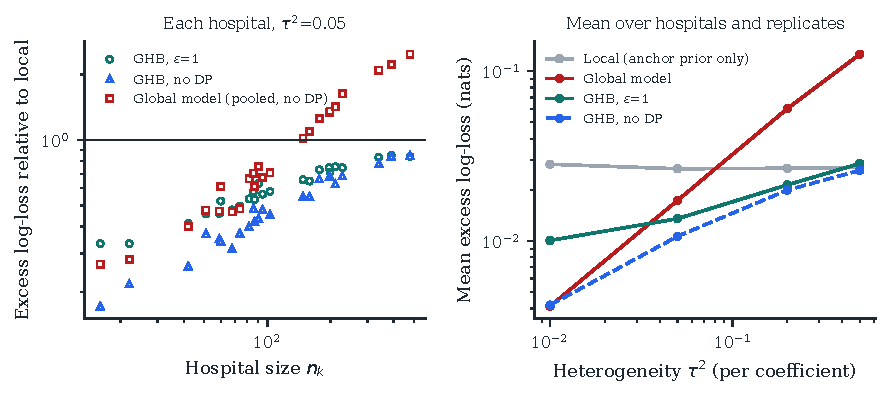
\includegraphics[width=\linewidth]{figures/s7_logistic}
\caption{Simulation 7. Left: excess log-loss relative to local estimation for each hospital ($\tau^2=0.05$). Right: mean excess log-loss against heterogeneity.}
\label{fig:s7}
\end{figure}

%% ===================================================================
\paragraph{Simulation 8: federated and meta-analytic baselines} The logistic world of Simulation 7, at $\epsilon=1$ and four levels of heterogeneity. All private methods use the same releases, so they satisfy the same guarantee: one-shot federated averaging \cite{mcmahan2017communication} (the sample-size weighted mean of the releases, one model for every hospital), the random-effects meta-analytic mean (DerSimonian-Laird \cite{dersimonian1986meta} weights, one model for every hospital), and a Ditto-style \cite{li2021ditto} personalized model, which fits each hospital's data with a proximal term $\frac{\lambda}{2}\|\theta-\bar{\theta}_{\mathrm{FedAvg }}\|^2$. The weight $\lambda$ is chosen from $\{0.3,1,3,10,30,100\}$ on ten separate tuning replicates per setting, which favours Ditto-style \cite{li2021ditto}. The global model fitted on the pooled data without privacy is a reference that no private method can match in general. Results (Figure~\ref{fig:s8}, left, and Table~\ref{M-tab:sim8} of the paper; 40 replicates per setting): at $\tau^2=0.05$, GHB-lite \SimEightMidGHB, Ditto-style \cite{li2021ditto} \SimEightMidDitto, pooled \SimEightMidPooled, meta-analysis \SimEightMidMeta, federated averaging \cite{mcmahan2017communication} \SimEightMidFedavg, local \SimEightMidLocal. At $\tau^2=0.5$, GHB-lite \SimEightHighGHB, Ditto-style \cite{li2021ditto} \SimEightHighDitto, local \SimEightHighLocal. One-shot federated averaging \cite{mcmahan2017communication} is weak here because it averages noisy releases without personalization; multi-round federated training with differentially private gradients is compared in Simulation 15.

\paragraph{Simulation 10: case-mix shift} As Simulation 8 at $\tau^2=0.05$, but each hospital draws its features from $\mathcal{N}(m_k,I)$ with $m_k\sim\mathcal{N}(0,s^2I)$, while the de-shrinking still uses the public, unshifted feature distribution (Figure~\ref{fig:s8}, right, and Table~\ref{M-tab:sim8} of the paper). At $s=1$: GHB-lite \SimEightShiftGHB, Ditto-style \cite{li2021ditto} \SimEightShiftDitto, pooled \SimEightShiftPooled, local \SimEightShiftLocal.

\begin{figure}[t]
\centering
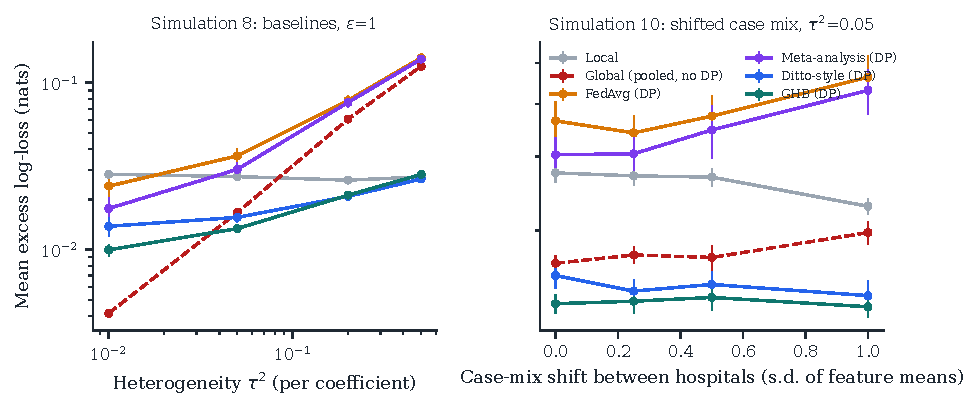
\includegraphics[width=\linewidth]{figures/sim8_baselines}
\caption{Simulations 8 and 10. Mean excess log-loss of GHB-lite and of private and non-private baselines against heterogeneity (left) and case-mix shift (right). Bars: $\pm2$ standard errors.}
\label{fig:s8}
\end{figure}

\paragraph{Simulation 9: atypical hospitals} The network of Simulation 2 at $\tau^2=0.02$ and $\epsilon=1$, with Gaussian site effects, Student-$t_3$ site effects of the same variance, or Gaussian effects plus one hospital at $u=6\tau$, placed at the smallest or at the largest hospital. Three estimators: Gaussian GHB-lite; robust GHB-lite, which replaces the Gaussian prior $\mathcal{N}(\tilde{\mu}_k,\hat{\tau}^2+M_k)$ by a Student-$t_3$ prior of the same variance (posterior mean by quadrature); and GHB-lite with opt-out, where a hospital keeps its local estimate when $|\hat{\theta}_k-\tilde{\mu}_k|/\sqrt{v_k+\hat{\tau}^2+M_k}>3$. Both variants change only the hospital's own computation and cost no privacy. Mean relative risk: Gaussian effects \SimNineGaussGHB{} (robust \SimNineGaussRobust), $t_3$ effects \SimNineTGHB{} (robust \SimNineTRobust). The outlying hospital: \SimNineSmallGHB{} (robust \SimNineSmallRobust, opt-out \SimNineSmallOpt) when it is the smallest, \SimNineLargeGHB{} (robust \SimNineLargeRobust) when it is the largest (Figure~\ref{fig:s9}; Tables~\ref{tab:s9} and~\ref{tab:s9bins}). With 16 patients, the standard error of the local estimate is as large as the deviation, so no test based on the hospital's own data can detect it reliably.

\begin{figure}[t]
\centering
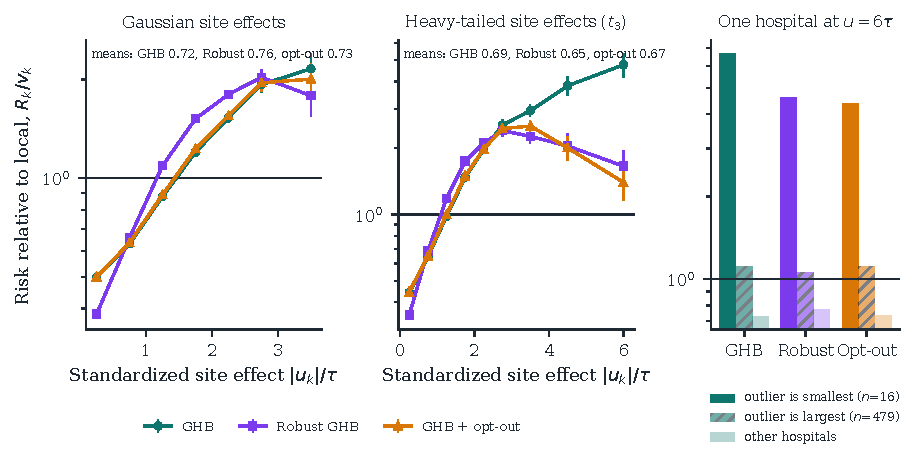
\includegraphics[width=\linewidth]{figures/sim9_atypical}
\caption{Simulation 9. Left and centre: relative risk against the standardized site effect for Gaussian and heavy-tailed effects. Right: the outlying hospital and the others, when the outlier is the smallest or the largest hospital.}
\label{fig:s9}
\end{figure}

\begin{table}[t]
\caption{Simulation 9: exact values behind Figure~\ref{fig:s9}, right. Mean relative risk; with an outlier, for the outlying hospital and for the others.}
\label{tab:s9}
\scriptsize
\begin{tabular}{@{}lrrrrrr@{}}
\toprule
& \multicolumn{3}{c}{All hospitals, or the outlier} & \multicolumn{3}{c}{The others}\\
\cmidrule(lr){2-4}\cmidrule(l){5-7}
Site effects & GHB-lite & Robust & Opt-out & GHB-lite & Robust & Opt-out\\
\midrule
\csname @@input\endcsname../../Collectively_Big_Locally_Small/supplement/results/tables/s_sim9.tex 
\bottomrule
\end{tabular}
\end{table}

\begin{table}[t]
\caption{Simulation 9: exact values behind Figure~\ref{fig:s9}, centre. Relative risk with Student-$t_3$ site effects, by standardized effect $|u_k|/\tau$, with two standard errors in grey; $N$: hospital-replicates in the bin.}
\label{tab:s9bins}
\scriptsize
\begin{tabular}{@{}lrrrr@{}}
\toprule
$|u_k|/\tau$ & GHB-lite & Robust & Opt-out & $N$\\
\midrule
\csname @@input\endcsname../../Collectively_Big_Locally_Small/supplement/results/tables/s_sim9_bins.tex 
\bottomrule
\end{tabular}
\end{table}


\paragraph{Simulation 11: a wrong anchor} The logistic world at $\tau^2=0.05$ and $\epsilon=1$, with the anchor wrong by $\mathcal{N}(0,e^2I)$ for $e$ from 0 to 3. GHB-lite uses the anchor with its uncertainty stated honestly ($e$), overconfidently (0.3 whatever $e$), overconfidently with a conflict check (the anchor is dropped when $|\mu_0-\tilde{\mu}_k|>3\sqrt{0.3^2+M_k}$ in any coordinate), or not at all. The local model uses $\mathcal{N}(\mu_0,I)$ as its prior and degrades with the anchor (Figure~\ref{fig:s11} and Table~\ref{tab:s11}). Honest uncertainty and the conflict check keep the excess log-loss at or below \SimElevenHonestMax{} at every error, GHB-lite without the anchor at or below \SimElevenNoAnchorMax; an overconfident anchor two standard deviations off reaches \SimElevenOverTwo, and local estimation \SimElevenLocalTwo.

\begin{figure}[t]
\centering
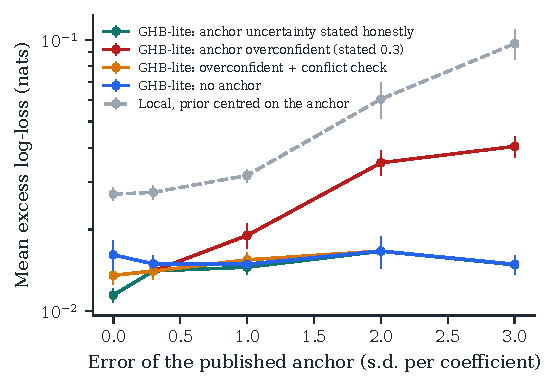
\includegraphics[width=0.62\linewidth]{figures/sim11_anchor}
\caption{Simulation 11. Mean excess log-loss against the error of the published anchor.}
\label{fig:s11}
\end{figure}

\begin{table}[t]
\caption{Simulation 11: exact values behind Figure~\ref{fig:s11}. Mean excess log-loss ($10^{-3}$ nats) against the standard deviation $e$ of the anchor's error, with two standard errors in grey; Honest: stated uncertainty $e$; Over.: stated 0.3; + check: stated 0.3 with the conflict check; Dropped: percentage of hospitals where the check drops the anchor.}
\label{tab:s11}
\scriptsize
\setlength{\tabcolsep}{4pt}
\begin{tabular}{@{}rllllll@{}}
\toprule
$e$ & Local & Honest & Over. & Over. + check & No anchor & Dropped (\%)\\
\midrule
\csname @@input\endcsname../../Collectively_Big_Locally_Small/supplement/results/tables/s_sim11.tex 
\bottomrule
\end{tabular}
\end{table}


\paragraph{Simulation 12: dishonest hospitals} The network of Simulation 2 at $\tau^2=0.02$ and $\epsilon=1$. The one or three largest hospitals release $\mu+b\tau$ instead of their privatized estimate; sizes are public, so they cannot change their weights. Robust GHB-lite obtains all releases by flooding, computes an inverse-variance weighted median and a MAD-based spread, drops releases more than three spreads away, and runs GHB-lite on the rest; this is post-processing. Honest hospitals' mean relative risk (Figure~\ref{fig:s12} and Table~\ref{tab:s12}): plain GHB-lite never exceeds \SimTwelveWorstGHB{}, because a large lie inflates $\hat{\tau}^2$ and switches borrowing off; robust GHB-lite keeps \SimTwelveRobustLarge{} against large lies, but costs \SimTwelveRobustNone{} against \SimTwelveGHBNone{} when nobody lies, because the screen sometimes drops honest outlying releases.

\begin{figure}[t]
\centering
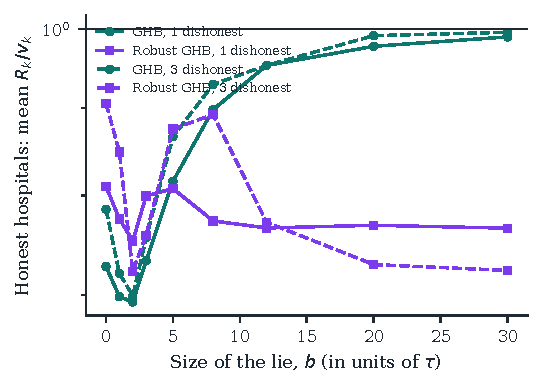
\includegraphics[width=0.62\linewidth]{figures/sim12_byzantine}
\caption{Simulation 12. Honest hospitals' mean relative risk against the size of the lie, for one and three dishonest hospitals.}
\label{fig:s12}
\end{figure}

\begin{table}[t]
\caption{Simulation 12: exact values behind Figure~\ref{fig:s12}. Honest hospitals' mean relative risk against the size $b$ of the lie (in units of $\tau$), and the percentage of dishonest releases that robust GHB-lite keeps.}
\label{tab:s12}
\footnotesize
\begin{tabular}{@{}rrrrrrr@{}}
\toprule
& \multicolumn{3}{c}{One dishonest hospital} & \multicolumn{3}{c}{Three dishonest hospitals}\\
\cmidrule(lr){2-4}\cmidrule(l){5-7}
$b$ & GHB-lite & Robust & Kept (\%) & GHB-lite & Robust & Kept (\%)\\
\midrule
\csname @@input\endcsname../../Collectively_Big_Locally_Small/supplement/results/tables/s_sim12.tex 
\bottomrule
\end{tabular}
\end{table}


\paragraph{Simulation 13: link failures} The network of Simulation 2 with every link failing independently in each round with probability $p$; the Metropolis-Hastings weights are recomputed on the working links, so each round's matrix stays symmetric and doubly stochastic. With $p=0.8$, the mean relative risk is \SimThirteenEightyTwenty{} after 20 rounds and \SimThirteenEighty{} after 60, against \SimThirteenExact{} with exact averaging (Figure~\ref{fig:s13} and Table~\ref{tab:s13}).

\begin{figure}[t]
\centering
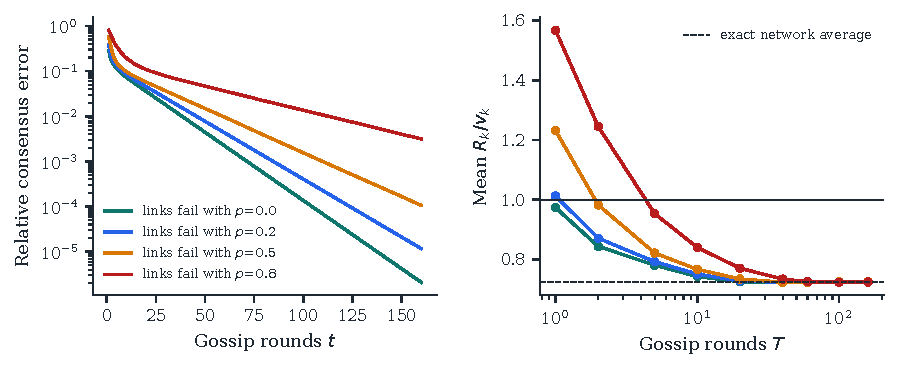
\includegraphics[width=\linewidth]{figures/sim13_dropout}
\caption{Simulation 13. Left: consensus error against rounds. Right: mean relative risk of plug-in GHB-lite against rounds, for four link-failure probabilities.}
\label{fig:s13}
\end{figure}

\begin{table}[t]
\caption{Simulation 13: exact values behind Figure~\ref{fig:s13}, right. Mean relative risk of plug-in GHB-lite after $T$ rounds, for link-failure probability $p$.}
\label{tab:s13}
\footnotesize
\begin{tabular}{@{}lrrrr@{}}
\toprule
$T$ & $p=0$ & $p=0.2$ & $p=0.5$ & $p=0.8$\\
\midrule
\csname @@input\endcsname../../Collectively_Big_Locally_Small/supplement/results/tables/s_sim13.tex 
\bottomrule
\end{tabular}
\end{table}


\paragraph{Simulation 14: repeated releases} For a total budget of $\epsilon=1$, $\delta=10^{-5}$ spread over $r$ refits on the same patients, the borrowed patients $B$ after the last refit (closed form, network of Simulation 2) under basic composition ($(\epsilon/r,\delta/r)$ per release) and under zero-concentrated accounting (the Gaussian mechanism with noise $s$ is $\rho$-zCDP with $\rho=\Delta^2/(2s^2)$; costs add; $\rho$-zCDP implies $(\rho+2\sqrt{\rho\ln(1/\delta)},\delta)$-DP). After \SimFourteenR{} refits, $B=\SimFourteenBasic$ under basic composition and \SimFourteenZcdp{} under zCDP, against \SimFourteenOne{} for a single release (Figure~\ref{fig:s14} and Table~\ref{tab:s14}).

\begin{figure}[t]
\centering
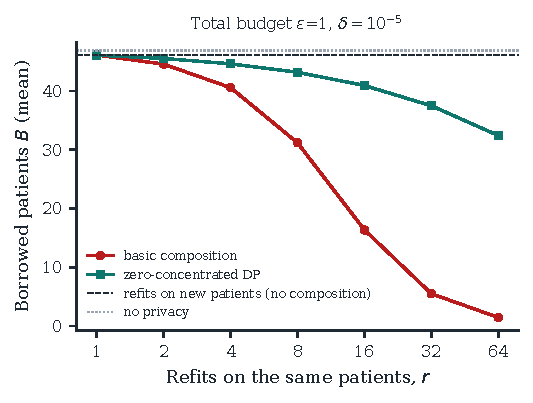
\includegraphics[width=0.62\linewidth]{figures/sim14_accounting}
\caption{Simulation 14. Borrowed patients after $r$ refits on the same patients, for a fixed total budget.}
\label{fig:s14}
\end{figure}

\begin{table}[t]
\caption{Simulation 14: exact values behind Figure~\ref{fig:s14}. Borrowed patients $B$ after $r$ refits for a total budget $\epsilon=1$, $\delta=10^{-5}$, under basic composition and zero-concentrated accounting, and the ratio of the per-release noise standard deviations (basic over zCDP).}
\label{tab:s14}
\footnotesize
\begin{tabular}{@{}lrrr@{}}
\toprule
$r$ & $B$, basic & $B$, zCDP & Noise ratio\\
\midrule
\csname @@input\endcsname../../Collectively_Big_Locally_Small/supplement/results/tables/s_sim14.tex 
\bottomrule
\end{tabular}
\end{table}


\paragraph{Simulation 15: iterative federated learning} The logistic world of Simulation 8 (24 hospitals, ring with two-hop links, $\delta=10^{-5}$), GHB-lite against multi-round training at the same privacy budget per hospital. GHB-lite is the revised version of Section~\ref{sec:revision}; the earlier version is reported alongside it. Per-patient gradients of the logistic loss are $(p-y)x$ with $\|x\|\le\sqrt{5}$, so they need no clipping, and replacing one patient moves a hospital's mean gradient by at most $2\sqrt{5}/n_k$. Every iterative method adds Gaussian noise to each hospital's mean gradient in every round and is accounted with zero-concentrated DP: with $R$ rounds, each round spends $\rho/R$, and the total $\rho$ satisfies $\rho+2\sqrt{\rho\ln(1/\delta)}=\epsilon$. GHB-lite's single release is accounted in the same way. All methods start from, or shrink toward, the published anchor $\mu_0$, which GHB-lite also uses.
\begin{itemize}[leftmargin=*,itemsep=1pt]
\item \emph{DP-FedAvg} \cite{mcmahan2017communication,mcmahan2018learning}, full-batch: a server holds one model; in each round every hospital sends its noisy mean gradient at that model, and the server takes a step of size $\eta$ along the sample-size weighted average.
\item \emph{DP-FedAvg \cite{mcmahan2018learning} with fine-tuning}: each hospital then takes $E$ plain gradient steps (step size 1) on its own data, starting from the global model; this costs no privacy because the data stay local.
\item \emph{Decentralized DP-SGD} \cite{lian2017can}, the algorithm behind swarm learning \cite{warnatherresthal2021swarm}: no server; each hospital steps along its own noisy gradient and averages models with its neighbours using the Metropolis-Hastings weights of GHB-lite's graph (adapt, then combine), followed by optional fine-tuning.
\item \emph{Clustered DP-FedAvg}, in the style of IFCA \cite{ghosh2020efficient}. IFCA \cite{ghosh2020efficient} lets each hospital choose the cluster whose model fits its data best in every round. Under DP this choice has sensitivity of order 1, not $1/n_k$, because one patient can move a hospital's whole gradient from one cluster to another. Hospitals therefore make one private ridge release with half the budget, the releases are clustered by weighted $k$-means (post-processing), and DP-FedAvg \cite{mcmahan2018learning} runs within each cluster with the other half, followed by optional fine-tuning.
\item \emph{Local gradient descent from the anchor}, a control that uses no other hospital: $E$ gradient steps on the hospital's own data from $\mu_0$, with early stopping as the only regularizer.
\item \emph{Ditto-style \cite{li2021ditto}} as in Simulation 8, and \emph{GHB-lite with the true $\tau^2$} (the marginal heterogeneity, regional plus within-region in the regional world), a reference that no method can use.
\end{itemize}
Hyperparameters are chosen on \SimFifteenTune{} separate replicates per setting by the mean excess log-loss, which requires access to the true models: rounds $R\in\{1,2,3,5,10,30,100\}$ ($\{3,10,30,100\}$ for decentralized training), step size $\eta\in\{0.2,0.5,2\}$, fine-tuning steps $E\in\{0,1,2,3,5,10,30,100\}$ and clusters $C\in\{2,3,4\}$. Table~\ref{tab:s15hyper} lists the choices. The only choices at the edge of a grid are $R=1$, the smallest meaningful number of rounds, and $\eta=0.2$ for decentralized training, where smaller steps would approach the anchor-only control. GHB-lite has no tuning parameter. Settings: $\tau^2\in\{0.01,0.05,0.2,0.5\}$ at $\epsilon=1$; $\epsilon\in\{0.3,\infty\}$ at $\tau^2=0.05$; a regional world in which the 24 hospitals form four regions, with between-region variance 0.2 and within-region variance 0.02 per coefficient, where clustering should help; an anchor wrong by $\mathcal{N}(0,I)$ instead of $\mathcal{N}(0,0.3^2I)$; $\tau^2=0.1$ at $\epsilon=0.5$; and a network of 48 hospitals (sizes drawn as for the 24, ring with two-hop links). The last four settings (marked $\ast$) were not used while revising GHB-lite; the development runs used other seeds, an anchor error of two standard deviations and a three-region world. Results are means over \SimFifteenReps{} further replicates (Table~\ref{tab:s15}, Figure~\ref{fig:s15}); Table~\ref{M-tab:sim15worst} of the paper gives the worst hospital, the share of hospitals that gain, and the largest hospitals.

GHB-lite is the most accurate private method in six of the ten settings ($\tau^2=0.01$ and $0.05$, $\epsilon=0.3$, and the held-out regional, $\tau^2=0.1$/$\epsilon=0.5$ and 48-hospital settings). The tuned Ditto-style \cite{li2021ditto} model, which shrinks toward the average of GHB-lite's own releases, is slightly more accurate at $\tau^2=0.2$, without privacy and with a wrong anchor; at $\tau^2=0.5$ no private method beats local estimation. GHB-lite is more accurate than DP-FedAvg \cite{mcmahan2018learning} with fine-tuning, decentralized DP-SGD \cite{lian2017can} and clustered training in every private setting. At $\epsilon=0.3$, the local control that starts from the anchor reaches \SimFifteenStrictAnchorGD{} against \SimFifteenStrictGHB{} for GHB-lite, and with a wrong anchor it becomes worse than local estimation (\SimFifteenAnchorAnchorGD{} against \SimFifteenAnchorLocal). GHB-lite's worst hospital is at most \SimFifteenGHBWorstMax{} times its local error in every private setting except $\tau^2=0.5$ (\SimFifteenExtremeGHBWorst), whereas fine-tuning's worst hospital is \SimFifteenFTWorstMin{} to \SimFifteenFTWorstMax{} times worse than alone; the hospitals that lose are the large ones. GHB-lite with the true $\tau^2$ remains better still (\SimFifteenStrictOracle{} at $\epsilon=0.3$), so estimating heterogeneity from noisy releases is what is left to improve. The earlier version of GHB-lite reached \SimFifteenStrictOld{} at $\epsilon=0.3$ and \SimFifteenMidOld{} at $\tau^2=0.05$.

\begin{table}[t]
\caption{Simulation 15. Mean excess log-loss (nats) over the hospitals and \SimFifteenReps{} replicates; lowest of the methods available to a hospital in bold (the earlier version of GHB-lite, the oracle and the pooled model are references). FT: fine-tuning. $\ast$: setting not used while revising GHB-lite.}
\label{tab:s15}
\scriptsize
\setlength{\tabcolsep}{3pt}
\resizebox{\linewidth}{!}{\begin{tabular}{@{}lrrrrrrrrrrr@{}}
\toprule
Setting & Local & \makecell[r]{Anchor\\GD} & GHB-lite & \makecell[r]{Ditto-\\style\\\cite{li2021ditto}} & \makecell[r]{DP-\\FedAvg\\\cite{mcmahan2018learning}} & \makecell[r]{DP-FedAvg\\+ FT\\\cite{mcmahan2018learning}} & \makecell[r]{Decentr.\\DP-SGD\\\cite{lian2017can}} & \makecell[r]{Clustered\\DP-FedAvg\\\cite{ghosh2020efficient}} & \makecell[r]{GHB-lite,\\earlier} & \makecell[r]{GHB-lite,\\true $\tau^2$} & \makecell[r]{Pooled,\\no DP}\\
\midrule
\csname @@input\endcsname../../Collectively_Big_Locally_Small/supplement/results/s15_table.tex 
\bottomrule
\end{tabular}}
\end{table}

\begin{table}[t]
\caption{Simulation 15. Hyperparameters chosen on the tuning replicates: rounds $R$, step size $\eta$, fine-tuning steps $E$, clusters $C$, and the proximal weight $\lambda$ of the Ditto-style \cite{li2021ditto} model.}
\label{tab:s15hyper}
\scriptsize
\resizebox{\linewidth}{!}{\begin{tabular}{@{}lllllr@{}}
\toprule
Setting & DP-FedAvg \cite{mcmahan2018learning} + FT & Decentralized DP-SGD \cite{lian2017can} & Clustered DP-FedAvg \cite{ghosh2020efficient} & Anchor GD & Ditto \cite{li2021ditto} $\lambda$\\
\midrule
\csname @@input\endcsname../../Collectively_Big_Locally_Small/supplement/results/s15_hyper.tex 
\bottomrule
\end{tabular}}
\end{table}

\begin{figure}[t]
\centering
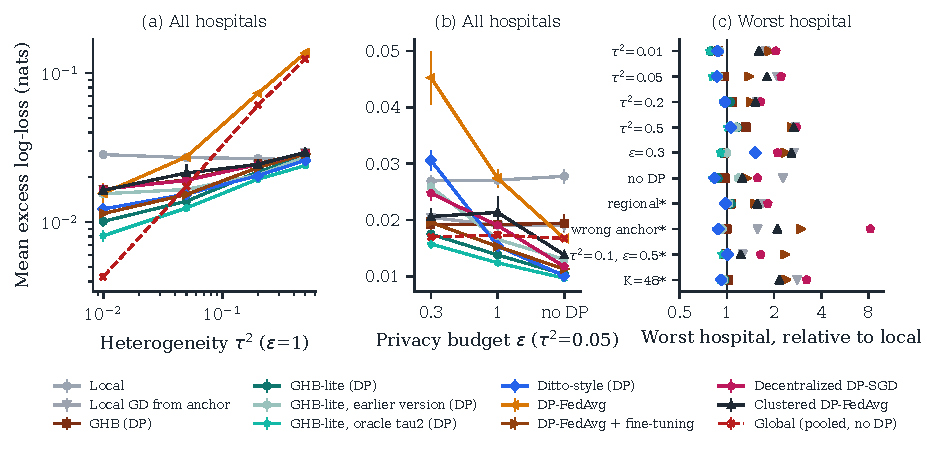
\includegraphics[width=\linewidth]{figures/sim15_literature}
\caption{Simulation 15. (a) Mean excess log-loss against heterogeneity at $\epsilon=1$. (b) Against the privacy budget at $\tau^2=0.05$. (c) The worst hospital's error relative to its own local estimate; right of 1, some hospital is worse off than alone. ``GHB-lite (DP)'' is GHB-lite and ``GHB (DP)'' is GHB with joint releases.}
\label{fig:s15}
\end{figure}

\paragraph{Simulation 16: ablation} The logistic world of Simulation 15 (24 hospitals, ring with two-hop links, $T=60$, $\delta=10^{-5}$), in eight settings: $\tau^2\in\{0.01,0.05,0.2,0.5\}$ at $\epsilon=1$; $\epsilon\in\{0.3,\infty\}$ at $\tau^2=0.05$; an anchor wrong by $\mathcal{N}(0,I)$; and a case-mix shift of one standard deviation. In every replicate, every variant uses the same data, the same public sample and the same standard-normal noise draw, scaled to its own noise level, so that differences between variants are paired. Each variant switches one component of GHB-lite (\texttt{simulations/ghb\_variants.py}, which reproduces the reported estimator to $10^{-10}$ with its default settings): the release (the sufficient statistic $X^\top y$, or a ridge fit with $\lambda=0.2$ centred on zero and undone at the leave-one-out point, instead of the score at the anchor); the second linearization; the rule for $\tau$ (plug-in posterior mean, posterior median or DerSimonian-Laird \cite{dersimonian1986meta}, or the posterior quantiles without weighting by the hospital's own evidence); the conflict check; the anchor; the default prior; inverse-variance weights in the network mean; gossip against exact averaging; and zero-concentrated against classical calibration of the noise. GHB-lite with the true $\tau^2$, the earlier version of GHB-lite and local estimation are references. Table~\ref{M-tab:sim16} of the paper gives the mean excess log-loss of each variant relative to GHB-lite over \SimSixteenReps{} replicates per setting. Part B repeats the ablation of the rule for $\tau$, the weights and the averaging in the Gaussian model of Simulation 2 over 20,000 replicates per setting (Table~\ref{tab:s16gauss}).
\begin{table}[t]
\caption{Simulation 16, part B: the Gaussian model. Mean relative risk $R_k/v_k$ over the 24 hospitals of Simulation 2 (20,000 replicates per setting). FB: $\tau$ integrated out with the hospital's own evidence (reported); Mean, DL: plug-in posterior mean and DerSimonian-Laird \cite{dersimonian1986meta}; No ev.: components without own evidence; Equal: equal weights; Exact: exact averaging; $T=10$: gossip with 10 rounds; Oracle: $\tau^2$ known.}
\label{tab:s16gauss}
\scriptsize
\resizebox{\linewidth}{!}{\begin{tabular}{@{}llrrrrrrrr@{}}
\toprule
$\tau^2$ & $\epsilon$ & FB & Mean & DL & No ev. & Equal & Exact & $T=10$ & Oracle\\
\midrule
\csname @@input\endcsname../../Collectively_Big_Locally_Small/supplement/results/s16_gauss_table.tex 
\bottomrule
\end{tabular}}
\end{table}

\paragraph{Simulation 17: sensitivity} Part A varies each setting of GHB-lite, the others at their reported values, in three base settings of the logistic world ($\tau^2=0.05$ at $\epsilon=1$ and $0.3$; $\tau^2=0.2$ at $\epsilon=1$), with every value computed on the same data and releases (\SimSeventeenReps{} replicates): the number of posterior quantiles of $\tau$, $Q\in\{1,3,6,12,24\}$ ($Q=1$ is the plug-in posterior median); the half-Cauchy scale of the prior on $\tau$, $\{0.1,0.25,0.5,1,2.5\}$; the standard deviation of the default prior, $\{1,2.5,5,10\}$ or none; the conflict threshold $z\in\{2,2.5,3,4,6\}$; the stated standard deviation of the anchor, $\{0.1,0.3,0.6,1,2\}$, whose true error is 0.3; the number of gossip rounds, $T\in\{5,10,20,40,60,120\}$; and the size of the public sample for the moments, $\{2{,}000,\,5{,}000,\,20{,}000,\,100{,}000\}$. Ranges of the ratio to the reported settings, over all values and base settings: $Q$ \SimSeventeenQMin{} to \SimSeventeenQMax; scale \SimSeventeenScaleMin{} to \SimSeventeenScaleMax; default prior \SimSeventeenPriorMin{} to \SimSeventeenPriorMax; threshold \SimSeventeenZMin{} to \SimSeventeenZMax; stated anchor uncertainty \SimSeventeenAnchorSdMin{} to \SimSeventeenAnchorSdMax; rounds \SimSeventeenTMin{} to \SimSeventeenTMax; public sample \SimSeventeenMMin{} to \SimSeventeenMMax. Part B varies, at $\tau^2=0.05$ and $\epsilon=1$, the number of hospitals ($K\in\{6,12,24,48,96\}$, sizes drawn as in Simulation 2), the median hospital size ($\{25,50,100,200,400\}$), the budget ($\epsilon\in\{0.1,0.2,0.3,0.5,1,2,5,\infty\}$, with zero-concentrated calibration, which is valid for every $\epsilon$), $\delta\in\{10^{-3},10^{-5},10^{-7},10^{-9}\}$ and the four topologies of Figure~\ref{M-fig:gossip} at $K=24$, each with its own seeds and \SimSeventeenReps{} replicates. GHB-lite's error relative to local estimation ranges from \SimSeventeenRelMin{} to \SimSeventeenRelMax, and its worst hospital stays within a factor \SimSeventeenWorstMax{} of its local error. Figures~\ref{M-fig:sim-settings} and~\ref{M-fig:sim-conditions} of the paper show every point, and Tables~\ref{M-tab:sim17a} and~\ref{M-tab:sim17b} give the values.

\paragraph{Simulations 16B and 17B: GHB} The ablation and sensitivity analysis of Simulations 16 and 17 repeated for GHB as released (\texttt{simulations/exp16b\_ghb.py} and \texttt{exp17b\_ghb.py}), in the same settings and conditions, with the published anchor (stated standard deviation 0.3) as in Simulation 15 and without the step across networks, since a simulated network is alone. Every variant of a replicate uses the same data and the same privacy noise (one seed per replicate, drawn from the data). Ablation: without the non-borrowing components; without the propagated privacy covariance; without removing the hospital's own data; intercept borrowed like the slopes; the loose (triangle-inequality) sensitivity of the information release; the full matrix or the diagonal always instead of the public rule; without the anchor. Sensitivity: half-Cauchy scale of $\tau$ in $\{0.1,0.25,1,2\}$, non-borrowing weight in $\{0.1,1,3\}$ (released $\frac13$), budget share of the information release in $\{0.25,0.75\}$, $Q\in\{1,3,6,24\}$, and default scales $\{2.5\}$, $\{1\}$ or $\{0.5,1,2.5,5\}$. Table~\ref{tab:s16b} gives every value behind Figure~\ref{M-fig:sim-ghb-ablation} of the paper; Figure~\ref{fig:s17b} and Table~\ref{tab:s17b} give GHB and GHB-lite across network conditions, on the same worlds.

\begin{table}[t]
\caption{Simulation 16B: ablation and sensitivity of GHB as released (\SimSixteenBReps{} replicates per setting). First row: mean excess log-loss of GHB ($10^{-3}$ nats). Other rows: the mean excess log-loss of each variant divided by that of GHB on the same data and privacy noise; bold where the paired difference exceeds two standard errors. Last row: local estimation.}
\label{tab:s16b}
\scriptsize
\setlength{\tabcolsep}{3pt}
\begin{tabular}{@{}lrrrrrrrr@{}}
\toprule
Variant & $\tau^2=0.01$ & $\tau^2=0.05$ & $\tau^2=0.2$ & $\tau^2=0.5$ & $\epsilon=0.3$ & no DP & \makecell[r]{wrong\\anchor} & shift\\
\midrule
\csname @@input\endcsname../../Collectively_Big_Locally_Small/supplement/results/tables/t_sim16_ghb.tex 
\bottomrule
\end{tabular}
\end{table}

\begin{figure}[t]
\centering
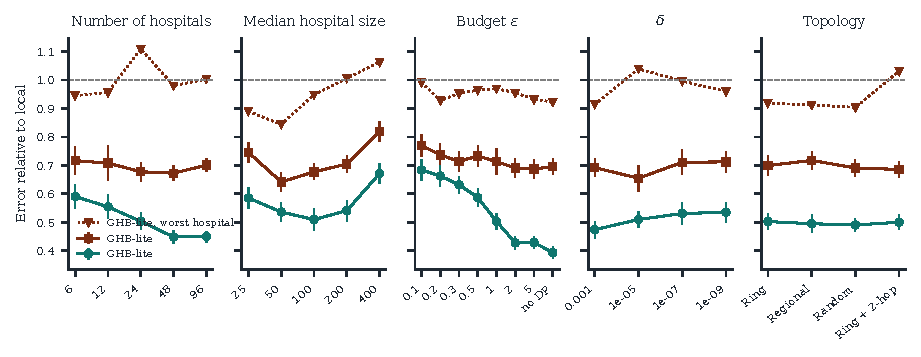
\includegraphics[width=\linewidth]{figures/sim17_ghb_conditions}
\caption{Simulation 17B: GHB as released and GHB-lite across network conditions, on the same worlds ($\tau^2=0.05$, $\epsilon=1$, 24 hospitals of median size 100 on the ring with two-hop links unless varied; 40 replicates per point). Mean excess log-loss relative to local estimation ($\pm2$ standard errors) and the largest ratio of any hospital's error to its own local error for GHB (dotted).}
\label{fig:s17b}
\end{figure}

\begin{table}[t]
\caption{Simulation 17B: exact values behind Figure~\ref{fig:s17b}. Mean excess log-loss of GHB and GHB-lite relative to local estimation, the largest ratio of any hospital's error to its own local error under GHB, and the absolute mean excess log-loss of GHB and of local estimation ($10^{-3}$ nats).}
\label{tab:s17b}
\scriptsize
\begin{tabular}{@{}llrrrrr@{}}
\toprule
Condition & Value & GHB / local & GHB-lite / local & Worst (GHB) & GHB & Local\\
\midrule
\csname @@input\endcsname../../Collectively_Big_Locally_Small/supplement/results/tables/s_sim17_ghb.tex 
\bottomrule
\end{tabular}
\end{table}

\paragraph{Simulation 18: group fairness} The logistic world of Simulation 7 ($\epsilon=1$, $\delta=10^{-5}$, 24 hospitals, ring with two-hop links, $T=60$) with features $x=(1,S,z_1,z_2,z_3)$: $S\in\{0,1\}$ is a protected attribute ($S=1$ the minority group) and $z\sim\mathcal{N}(0,I_3)$ is clipped to $\|z\|\le\sqrt{3}$, so that $\|x\|\le\sqrt{5}$ and the sensitivity of the release is unchanged. Hospital $k$'s minority share is $\pi_k\sim\mathrm{Beta}(6\bar\pi,6(1-\bar\pi))$, clipped to $[0.02,0.98]$, with $\bar\pi=0.3$ (0.1 in the rare-minority scenario); the public feature distribution used for the inversion has share $\bar\pi$, so hospitals whose share differs are under case-mix shift. $\theta_k=\mu+u_k$ with $\mu=(-0.5,\mu_S,0.8,-0.6,0.4)$, $u_k\sim\mathcal{N}(0,\mathrm{diag}(\tau^2,\tau_S^2,\tau^2,\tau^2,\tau^2))$, $\tau^2=0.05$, and $(\mu_S,\tau_S^2)=(0.5,0.05)$ (shared), $(0.5,0.5)$ (varies), $(0.5,0.05)$ with $\bar\pi=0.1$ (rare) or $(0,0.5)$ (opposite); the anchor is $\mu$ plus $\mathcal{N}(0,0.3^2I)$. \emph{GHB-lite, $S$ local} replaces, in every mixture component of each hospital's prior, the network estimate of the coefficient of $S$ and its variance by the local prior $\mathcal{N}(\mu_{0,S},1)$. FAIR-FATE follows Algorithm~1 of \cite{salazar2023fairfate} with the settings in the caption of Table~\ref{M-tab:sim18} of the paper; the fairness of a model on the server's validation set is its SP, EO or EQO ratio at threshold 0.5, in the form $\min(a,b)/\max(a,b)$, and EQO averages the ratios of true and false positive rates. The validation set holds a quarter as many patients as each hospital's training data, drawn from that hospital's distribution, so a fifth of all patients, as in the paper. Each method is evaluated on 4,000 new patients per hospital, drawn from the hospital's own distribution; the fairness ratios are computed on the pooled test patients of all hospitals, each scored by the model its hospital uses. Results over \SimEighteenReps{} replicates per scenario are in Table~\ref{M-tab:sim18} and Figure~\ref{M-fig:sim-fairness} of the paper. The code is \texttt{simulations/exp18\_fairness.py}.

\section{Real Data: TCGA Design, Ablation and Held-Out Networks}\label{sec:tcga}

\paragraph{Data} Open-access clinical data of The Cancer Genome Atlas \cite{weinstein2013cancer,grossman2016toward} from the NCI Genomic Data Commons (\url{https://api.gdc.cancer.gov/cases}, script \texttt{simulations/fetch\_tcga.py}, files in \texttt{data/tcga\_v3/} and \texttt{data/tcga\_v4/}), downloaded with the fields vital status, days to death, age at index, sex at birth, days to last follow-up, AJCC pathologic stage, T and N, FIGO stage, prior malignancy, primary-diagnosis flag and the tissue source site. A hospital is a tissue source site (by name) with at least five eligible patients. A patient is eligible with a known age, sex and pathologic stage (AJCC, or FIGO where AJCC is absent), and a two-year outcome: death within 730 days, or known survival beyond it.

\paragraph{Model} $x=(1,a,\text{male},\text{stage III},\text{stage IV},\text{T3 or T4},\text{N1 to N3},\text{prior malignancy})$ with $a=(\text{age}-62)/25$ clipped to $[-1,1]$, so $\|x\|\le\sqrt{8}$ without fitting anything to the data. Stage letters and digits are dropped (IIIC1 is III).

\paragraph{Sets} Design: LUSC, HNSC, BLCA, STAD, LIHC, KIRC (the first set), and LUAD, COAD, READ, KIRP, PAAD, ESCA (the second set). Held out: every further TCGA project with at least four hospitals and at least fifteen deaths, fixed from counts alone before any model was fitted: BRCA, MESO, UCEC, OV and UCS. Of the other projects with downloadable data, ACC, PRAD and CESC have no or too few eligible hospitals, and THCA, KICH and TGCT too few deaths.

\paragraph{Protocol} Ten repetitions of five-fold cross-validation, stratified by outcome within each hospital, with the networks of a set fitted jointly so that GHB can borrow across them; every other method is fitted per network. Budgets $\epsilon\in\{1,10\}$, $\delta=10^{-5}$, zero-concentrated accounting. Errors are pooled held-out log-loss over repetitions and hospitals, relative to local estimation under $\mathcal{N}(0,2.5^2)$. The baselines and their grids are in Table~\ref{tab:tcga-configs}. Script \texttt{simulations/real\_v3.py} (sets \texttt{dev}, \texttt{fresh}, \texttt{confirm}), with checkpoints per repetition.

\begin{table}[t]
\caption{TCGA: the literature methods, the size of each grid, and the configuration with the lowest mean error over the twelve design networks, fixed before the held-out run (\texttt{dev/v4\_realistic\_configs.json}). Every method spends the same budget, with private gradients under zero-concentrated accounting.}
\label{tab:tcga-configs}
\scriptsize
\begin{tabularx}{\linewidth}{@{}lr>{\raggedright\arraybackslash}X>{\raggedright\arraybackslash}X@{}}
\toprule
Method & Grid & $\epsilon=1$ & $\epsilon=10$\\
\midrule
\csname @@input\endcsname../../Collectively_Big_Locally_Small/supplement/results/tables/s_tcga_configs.tex 
\bottomrule
\end{tabularx}
\end{table}

\begin{table}[t]
\caption{TCGA development: twelve networks, ten repetitions; held-out log-loss relative to local estimation, mean over the networks. GHB and GHB-lite with the evidence-weighted default prior. Literature methods: tuned on the same twelve networks (development tuning, in sample, which favours them) and on each network's own held-out folds (oracle).}
\label{tab:tcga-dev}
\scriptsize
\begin{tabular}{@{}lrrrr@{}}
\toprule
 & \multicolumn{2}{c}{$\epsilon=1$} & \multicolumn{2}{c}{$\epsilon=10$}\\
\cmidrule(lr){2-3}\cmidrule(l){4-5}
Method & Development & Oracle & Development & Oracle\\
\midrule
\csname @@input\endcsname../../Collectively_Big_Locally_Small/supplement/results/tables/s_tcga_dev.tex 
\bottomrule
\end{tabular}
\end{table}

\begin{table}[t]
\caption{TCGA held-out networks: every literature method in the oracle arm, tuned on each network's own held-out folds; relative held-out log-loss. Compare with Table~\ref{M-tab:tcga-confirm} of the paper.}
\label{tab:tcga-oracle}
\scriptsize
\begin{tabular}{@{}lrrrrrr@{}}
\toprule
Method & BRCA & MESO & OV & UCEC & UCS & Mean\\
\midrule
\csname @@input\endcsname../../Collectively_Big_Locally_Small/supplement/results/tables/s_tcga_oracle.tex 
\bottomrule
\end{tabular}
\end{table}

\paragraph{Design of GHB} GHB's joint releases were selected among about fifteen variants on the design networks (\texttt{simulations/dev/v4\_dev.py}, with the folds of \texttt{real\_v3.py}). Iterating the releases as Newton's method, with the information released at every iterate, was dominated by noise at $\epsilon=10$, because a Newton step divides the noise by the information of rare features. Releasing the information once, at the origin, propagating the privacy covariance into each hospital's prior and borrowing across networks fixed this; Table~\ref{M-tab:tcga-ablation} of the paper gives what each component of GHB as released contributes. One Newton step was better than two, which spend half the budget per step; learning $\tau$ from per-hospital releases at half the budget did not help; institution effects across networks changed the third decimal at most.

\begin{table}[t]
\caption{Tuned against tuned, on the five held-out networks, for GHB as released: mean held-out log-loss relative to local estimation. GHB tuned over \SimTTConfigs{} configurations, every literature method over its grid of 12 to 54. Development: the configuration with the lowest mean error over the twelve development networks, applied unchanged. Oracle: the best configuration on each network's own held-out folds. pFedMe with its correct privacy calibration.}
\label{tab:tcga-tuned}
\scriptsize
\begin{tabular}{@{}lrrrr@{}}
\toprule
 & \multicolumn{2}{c}{$\epsilon=1$} & \multicolumn{2}{c}{$\epsilon=10$}\\
\cmidrule(lr){2-3}\cmidrule(l){4-5}
Method & Development & Oracle & Development & Oracle\\
\midrule
\csname @@input\endcsname../../Collectively_Big_Locally_Small/supplement/results/tables/t_tcga_tuned.tex 
\bottomrule
\end{tabular}
\end{table}


\paragraph{Design choices} Three choices were made on the design networks (\texttt{simulations/dev/v5\_dev.py}), the seven small networks and UCI Heart Disease (\texttt{dev/v5\_networks.py}), and FLamby, and never on the five held-out networks; an earlier configuration, which borrowed the intercept, had been evaluated on those networks before, so its results on them were known when these choices were made. Not borrowing the intercept (an extra prior variance $2.5^2$ around the network value, and a default intercept scale of 2.5 whatever the scale of the slopes) improved the design networks from 0.934 to 0.923 of the local error at $\epsilon=1$ and from 0.913 to 0.899 at $\epsilon=10$ (four repetitions), and, together with the other two choices, Fed-Heart-Disease at $\epsilon=10$ from 0.440 to 0.427. The tighter sensitivity of the information release is a free improvement of the same guarantee. The diagonal fallback improved the design networks at $\epsilon=1$ (to 0.915, four repetitions) and Fed-TCGA-BRCA at $\epsilon=1$, where the full matrix of 40 coefficients is mostly noise. Rejected: weighting the components by their leave-one-out predictive accuracy (better on Fed-Heart-Disease by about 0.01, worse on the design networks by 0.003 and on the small networks by 0.004); a noise-aware network estimate (better at $\epsilon=1$, worse at $\epsilon=10$ by 0.009); approximating the network's information by each hospital's own; off-diagonal shrinkage of the released matrix; several damped Newton rounds; and, for images, borrowing only along leading public directions.

\paragraph{Not borrowing the intercept in simulation} In Simulation 16B, borrowing the intercept like the slopes would lower GHB's error to as little as \SimSixteenBIntMin{} of the released version's ($\tau^2=0.01$), and would raise it slightly at $\tau^2=0.5$ (\SimSixteenBIntMax): the simulated hospitals differ in base rate no more than in slopes. Letting each hospital's evidence decide, with every component present twice, intercept borrowed and not, each with half the weight (\texttt{int\_mix} in \texttt{ghb\_v4.py}), keeps most of the real-data gain on the design networks (0.920 and 0.901 at $\epsilon=1$ and 10, against 0.915 and 0.897 for GHB as released in the same four-repetition runs, \texttt{dev/v5\_dev.py}). It is not part of GHB and has not been evaluated on held-out data.

\paragraph{Tuning GHB} GHB as released was also tuned like the literature methods (Table~\ref{tab:tcga-tuned}; \texttt{simulations/dev/v5\_tune.py}), over \SimTuneConfigs{} configurations: the half-Cauchy scale of $\tau$ in $\{0.1,0.25,0.5,1\}$, the weight of the non-borrowing components in $\{0,\frac13,1\}$ and the share of the budget for the information release in $\{\frac14,\frac12,\frac34\}$ (released $(0.5,\frac13,\frac12)$), with shared folds and privacy noise. On the five held-out networks the released configuration reaches \SimTuneOneFixed{} and \SimTuneTenFixed{} at $\epsilon=1$ and 10; the configuration best on the design networks reaches \SimTuneOneDev{} and \SimTuneTenDev, and the best on each held-out network's own folds \SimTuneOneOrc{} and \SimTuneTenOrc.

\section{Real Data: The FLamby Benchmark}\label{sec:flamby}

\paragraph{Protocol} FLamby \cite{ogierduterrail2022flamby}, code at commit \texttt{edacf54}; script \texttt{simulations/flamby\_bench.py}, results \texttt{supplement/results/flamby\_results.json}. FLamby's preprocessing and static splits were reimplemented in NumPy and pandas and checked against its documentation: Fed-Heart-Disease has 199/104, 172/89, 30/16 and 85/45 training and test patients in Cleveland, Hungary, Switzerland and Long Beach; Fed-TCGA-BRCA has 248/63, 156/40, 164/42, 129/33, 129/33 and 40/11 in its six regions. Twenty runs per method, at $\epsilon\in\{1,10\}$ and without privacy, $\delta=10^{-5}$; the mean over hospitals of each hospital's test metric, as FLamby reports it.

\paragraph{Models} Heart: logistic regression on FLamby's 13 features, standardized with each hospital's training statistics, divided by 3 and clipped to $[-1,1]$, so $\|x\|\le\sqrt{14}$ with the intercept. TCGA-BRCA: an exponential survival model, the Poisson regression with per-patient log-likelihood $d\eta-t e^{\eta}$, follow-up $t$ in units of ten years clipped to $[0,1]$; the 38 binary columns are the one-hot coding of 14 variables, a public schema, so $\|x\|\le4$ with the intercept and the continuous age. GHB's joint releases use the score $x(d-t)$ at the origin, with sensitivity $2G$, and the information $t\,xx^\top$, with Frobenius sensitivity $\sqrt2\,G^2$ (the bound for positive semidefinite rank-one terms of Section~\ref{M-sec:logit}); the literature methods clip each patient's gradient to norm $G$, which is the gradient of a convex loss, so their sensitivity arguments carry over. The new code (\texttt{simulations/ghb\_glm.py}) reproduces the logistic originals exactly on every configuration.

\paragraph{Notes} GHB-lite was not run on TCGA-BRCA (its public-moment inversion needs a public model of follow-up and censoring); the TCGA-BRCA feature bound is 4 rather than $\sqrt{40}$, for the reason above; in the Poisson version of GHB, each maximum a posteriori fit starts from the better of the prior mean and the origin, which leaves the maximum unchanged because the objective is convex, and components whose Laplace evidence is not finite receive zero weight; the oracle is chosen separately for each metric. Fed-ISIC2019 uses FLamby's encoder (EfficientNet-B0 of \texttt{efficientnet\_pytorch}, ImageNet weights from the package's GitHub release, checksum-verified); with the tabular head, its features were projected to 16 dimensions with a public random matrix, and each of the eight classes had a one-vs-rest logistic head with an eighth of the budget.

\paragraph{Fed-ISIC2019} Balanced accuracy (FLamby's metric), mean over the six centres and 20 runs: a hospital alone 0.300, with the evidence prior 0.303, the pooled model 0.250; GHB 0.300, 0.299 and 0.300 at $\epsilon=1$, $10$ and without privacy; Ditto \cite{li2021ditto} 0.296, DP-FedAvg \cite{mcmahan2018learning} with fine-tuning and secure aggregation \cite{bonawitz2017practical} 0.207 and pFedMe \cite{tdinh2020personalized} 0.225 at $\epsilon=10$. With this weak projection every method that borrows stays at the local level, and the federated-averaging methods fall below it. The image version of GHB (Section~\ref{sec:images}) was designed on this dataset.


\section{Real Data: Images}\label{sec:images}

\paragraph{Model} Scripts \texttt{simulations/ghb\_image.py} (the method and the multinomial literature baselines), \texttt{isic\_image.py} (design) and \texttt{camelyon\_image.py} with \texttt{camelyon\_slides.py} (held-out evaluation). Encoder: EfficientNet-B0 \cite{tan2019efficientnet} from \texttt{efficientnet\_pytorch}, the encoder of FLamby's ISIC baseline \cite{ogierduterrail2022flamby}, with its ImageNet weights (\texttt{efficientnet-b0-355c32eb.pth}, SHA-256 checked), frozen; features are the 1,280 outputs of the global average pool. Projection: the first 32 principal components of the public images' features; each hospital standardizes the projected features with its training statistics, divides by 3 and clips to $[-1,1]$, so $\|x\|\le G=\sqrt{33}$ with the intercept. Head: softmax over $K$ classes, $\theta\in\mathbb{R}^{33\times K}$; a patient's score $x(e_y-p)^\top$ has Frobenius norm at most $\sqrt2\,G$, so a replacement moves a score sum by at most $2\sqrt2\,G$, the sensitivity used by GHB and every literature method. GHB: a share 0.05 of the budget releases the class counts (sensitivity $\sqrt2$), which start the intercepts at the centred log frequencies; one damped Newton round releases the secure sum of the scores at that point, with the curvature $N\,\mathbb{E}_{\text{pub}}[(\operatorname{diag}p-pp^\top)\otimes xx^\top]$ from the public images ($N$ is public under replacement) and each step projected on parameters whose rows sum to zero across classes, the softmax's invariance. Each hospital then forms its leave-one-out prior from the released sum, its own score and information and the public curvature, and averages the fits under the half-Cauchy components and the non-borrowing components by their evidence, as in Section~\ref{M-sec:logit} of the paper. Every method predicts $\arg\max_k s_k-\log\pi_k$ \cite{menon2021longtail}, with $\pi$ the mean predicted class probability on the hospital's own training images, over the classes it has seen.

\paragraph{Design (ISIC 2019)} FLamby's Fed-ISIC2019 \cite{combalia2019bcn20000}, its six centers and fixed splits; public images for the projection and the curvature: the 8,238 ISIC 2019 Test images, unlabeled. Variants tried: one or four Newton rounds, damping, free intercepts, borrowing along fewer public directions, the projection dimension. Chosen: one round, the class-count start, the intercept handled by the logit adjustment, all 32 directions. \SimIsicImgReps{} repetitions. pFedMe's rows use its corrected noise.

\paragraph{Held-out evaluation (Camelyon17)} Camelyon17-WILDS \cite{koh2021wilds} is distributed only from \texttt{worksheets.codalab.org}, whose TLS certificate had expired when this study ran; mirrors were not reachable from the computing environment. The patches were therefore rebuilt from the organizers' release of CAMELYON17 \cite{bandi2019camelyon17} (AWS Open Data) with the WILDS preprocessing code (commit \texttt{4726775}): the 50 slides with lesion annotations, ten per center; 96-pixel patches at level 2 on a 32-pixel grid; a patch is tumor if its central region touches a tumor polygon and normal if more than 20\% of it is non-tumor tissue (Otsu threshold of the saturation at level 4); per-slide and per-center class balancing with WILDS's seed. Slides were read by HTTP range requests (\texttt{tifffile}) instead of OpenSlide from a local copy; the annotation files matched their MD5 checksums. The rebuilt metadata has 29,717, 17,452, 42,527, 64,919 and 72,726 tumor patches (and as many normal) in centers 0 to 4, against 29,718, 17,452, 42,527, 64,919 and 73,361 in the released Camelyon17-WILDS; the difference in center 4 comes from one slide with more tumor than normal tissue. Pool: 600 tumor and 600 normal patches per hospital (fixed seed); each repetition splits each hospital's pool, stratified, into 200 training and 1,000 test patches. Public images: 200 tissue patches from each of ten slides of the challenge's test set (patients 100 to 199, ten distinct patients drawn with a fixed seed), unlabeled. Encoder input: the patch resized to $224\times224$, ImageNet normalization. Ten repetitions, $\epsilon\in\{1,10\}$ and no privacy, $\delta=10^{-5}$; realistic arm \texttt{dev/v4\_realistic\_configs.json}, oracle arm the best configuration per family and budget by the repetition-averaged mean. Balanced accuracy and log-loss per hospital, mean over hospitals. The privacy unit is a patch.

\begin{table}[ht]
\centering
\caption{Camelyon17 (held-out evaluation): balanced accuracy (higher is better) and log-loss of the logit-adjusted probabilities (lower is better), mean over five hospitals and \SimCamReps{} repetitions. Bold: the best per column among methods that use other hospitals, oracle excluded. $\dagger$: not private. $\star$: best of the six methods on the test patches. pFedMe's correctly calibrated noise makes it diverge at $\epsilon\in\{1,10\}$.}
\label{tab:camelyon}
\resizebox{\linewidth}{!}{\begin{tabular}{@{}lrrrrrr@{}}
\toprule
 & \multicolumn{3}{c}{Balanced accuracy} & \multicolumn{3}{c}{Log-loss}\\
\cmidrule(lr){2-4}\cmidrule(l){5-7}
Method & $\epsilon=1$ & $\epsilon=10$ & no privacy & $\epsilon=1$ & $\epsilon=10$ & no privacy\\
\midrule
\csname @@input\endcsname ../../Collectively_Big_Locally_Small/supplement/results/tables/s_camelyon.tex 
\bottomrule
\end{tabular}}
\end{table}

\paragraph{Results} At $\epsilon=10$ GHB was above a hospital alone in every repetition and above every realistic literature method, by 0.0015 to 0.0021 over the four closest (about one to three and a half paired standard errors, the lead over Ditto \cite{li2021ditto} being the clearest); at $\epsilon=1$ it was above a hospital alone and slightly below DP-FedAvg with fine-tuning; without privacy it was above a hospital alone and the pooled model; its log-loss at $\epsilon=10$ was lower than local. Over the local model with the evidence-weighted prior, GHB gained 0.0036 of balanced accuracy at $\epsilon=10$, in all ten repetitions; Ditto (realistic) matched its log-loss.

\section{Re-identification Risk}\label{sec:reid}

\paragraph{Bound} GHB's two releases are Gaussian mechanisms with half of a zero-concentrated budget $\rho$ each, so together they are $\mu$-Gaussian differentially private with $\mu=\sqrt{2\rho}$ \cite{dong2022gaussian}: for any test of whether a given patient's record was used (against any replacement record), the true-positive rate at false-positive rate $\alpha$ is at most $\Phi(\Phi^{-1}(\alpha)+\mu)$, and the advantage, true-positive minus false-positive rate, at most $2\Phi(\mu/2)-1$. With $\delta=10^{-5}$, $\mu=\SimReidOneMu$ at $\epsilon=1$ and $\mu=\SimReidTenMu$ at $\epsilon=10$; the largest true-positive rate at a 10\% false-positive rate is \SimReidOneTprTen{} and \SimReidTenTprTen.

\paragraph{Realized risk} For each of the \SimReidPatients{} patients of the 17 TCGA networks, the attainable $\mu_i$ is the norm of the change that replacing the patient's record by another patient's of the same network makes to the two sums, each divided by its noise standard deviation, maximized over the replacements; the patient's attainable advantage is $2\Phi(\mu_i/2)-1$ (\texttt{simulations/reid\_risk.py}).

\paragraph{Likelihood-ratio attack} The realized advantage is the power of the Neyman-Pearson test of an attacker who knows every other record and sees both raw releases: whitened by the noise, the releases differ by a known vector of norm $\mu_i$, so the test thresholds their projection on it. Simulating it for \SimReidLRPatients{} patients drawn at random from the 17 networks, with 4,000 releases with and without each patient, gives an advantage of \SimReidOneLRAdv{} at $\epsilon=1$ and \SimReidTenLRAdv{} at $\epsilon=10$, against \SimReidOneLRAna{} and \SimReidTenLRAna{} calculated, and true-positive rates at a 1\% false-positive rate of \SimReidOneLRTpr{} and \SimReidTenLRTpr.

\paragraph{Loss-threshold attack} A loss-threshold membership-inference attack \cite{shokri2017membership}: members are the training patients of a fold, non-members the held-out patients of the same hospitals; the attacker scores each patient by minus its log-loss under the released model, and the AUC of that score measures what it learns (0.5: nothing). Five repetitions, one random fold each, all 17 networks. Each hospital's own model is fitted with the default prior; the pooled network model by maximum a posteriori on all training patients; GHB's released network estimate is the one Newton step from its two releases (Section~\ref{M-sec:logit}). For each hospital's own model the AUC pools the members and non-members of all hospitals of a size band, since a small hospital's held-out fold has only one to three patients.

\begin{table}[ht]
\centering
\caption{Membership-inference attack on the 17 TCGA networks: AUC of telling training from held-out patients by their loss under each released model (0.5: no information).}
\label{tab:reid-attack}
\scriptsize
\begin{tabular}{@{}lr@{}}
\toprule
Released model & AUC\\
\midrule
\csname @@input\endcsname../../Collectively_Big_Locally_Small/supplement/results/tables/s_reid_attack.tex 
\bottomrule
\end{tabular}
\end{table}

\section{Real Data: Seven Smaller Networks}\label{sec:eight}

These tables give every network's result behind Table~\ref{M-tab:real-final} of the paper, in the leave-one-network-out arm: every literature method uses the configuration with the lowest mean error over the other networks. Medicare is Arizona Medicare (43 hospitals); the TCGA networks use the five-coefficient head of the paper and are fitted one at a time. Values are held-out log-loss relative to local estimation; bold marks the lowest per network among methods that use other hospitals.

\begin{table}[t]
\caption{Seven small networks, $\epsilon=1$, leave-one-network-out arm: held-out log-loss relative to local estimation, per network.}
\label{tab:eight-eps1}
\scriptsize
\setlength{\tabcolsep}{2.4pt}
\begin{tabular}{@{}lrrrrrrr@{}}
\toprule
 & Medicare & LUSC & HNSC & BLCA & STAD & LIHC & KIRC\\
\midrule
\csname @@input\endcsname ../../Collectively_Big_Locally_Small/supplement/results/tables/s_real_final_lono_eps1.tex 
\bottomrule
\end{tabular}
\end{table}

\begin{table}[t]
\caption{Seven small networks, $\epsilon=10$, leave-one-network-out arm: held-out log-loss relative to local estimation, per network.}
\label{tab:eight-eps10}
\scriptsize
\setlength{\tabcolsep}{2.4pt}
\begin{tabular}{@{}lrrrrrrr@{}}
\toprule
 & Medicare & LUSC & HNSC & BLCA & STAD & LIHC & KIRC\\
\midrule
\csname @@input\endcsname ../../Collectively_Big_Locally_Small/supplement/results/tables/s_real_final_lono_eps10.tex 
\bottomrule
\end{tabular}
\end{table}

\section{Real Data: UCI Heart Disease}\label{sec:real}

\paragraph{Data} The processed Cleveland, Hungarian, Switzerland and VA Long Beach files of the UCI Heart Disease data \cite{detrano1989international} (CC BY 4.0), as distributed by the UCI Machine Learning Repository; they are in \texttt{data/heart\_disease/} of the repository. The outcome is angiographic coronary disease ($\text{num}>0$). Sizes and prevalences: Cleveland 303 (46\%), Budapest 294 (36\%), Zurich and Basel 123 (93\%), Long Beach 200 (75\%). Age, sex and chest-pain type are complete at every site; the exercise-test variables are missing for about a quarter of the Long Beach patients, and cholesterol is recorded as zero at the Swiss sites, so they are not used.

\paragraph{Model and privacy} $x=(1,a,\text{male},\text{asymptomatic},\text{anginal})$ with $a=(\text{age}-55)/25$ clipped to $[-1,1]$; non-anginal pain is the reference, and anginal combines typical and atypical angina. Hence $\|x\|\le 2\le\sqrt{5}$, and the release (the mean score at 0, $\epsilon\in\{1,5\}$, $\delta=10^{-5}$, zero-concentrated calibration) has the sensitivity used throughout. GHB-lite is \texttt{ghb\_logit.py} without an anchor: the conflict check is off, the second linearization point is the leave-one-out network estimate combined with the default prior $\mathcal{N}(0,2.5^2)$ in place of an anchor (without it, the linearization point of a hospital with 20 patients can reach the clipping bound and make the public information matrix singular), and the final fit uses only the network components and the default prior. The public feature distribution is age $\mathcal{N}(55,9^2)$, male with probability 0.75 and chest pain asymptomatic, anginal or non-anginal with probabilities 0.5, 0.3 and 0.2, independently: a nominal referral population, not estimated from the data. With the public information at 0, the standard deviation of the privacy noise on the parameter scale is, at the median coefficient, 26 times the sampling standard error of a hospital of 40 patients at $\epsilon=1$, 5.6 times at $\epsilon=5$, and 9.5 and 2.0 times for a hospital of 300 patients.

\paragraph{Evaluation} Twenty repeats of stratified five-fold cross-validation within each hospital, with the folds of the four hospitals aligned so that every split has one training set and one test set per hospital. The training set is subsampled, stratified by outcome, to at most 20, 40 or 80 patients, or kept whole. All methods are fitted on the training sets and scored on each hospital's own test fold by log-loss, Brier score and AUC. Baselines (\texttt{simulations/literature.py}): DP-FedAvg \cite{mcmahan2018learning} from 0 with $R\in\{1,3,10,30\}$ rounds, step $\eta\in\{0.2,0.5,2\}$ and $E\in\{0,1,5,30\}$ full-batch fine-tuning steps of size 1; the Ditto-style \cite{li2021ditto} model, a MAP fit with prior $\mathcal{N}(\bar\theta,\lambda^{-1}I)$ around the size-weighted mean $\bar\theta$ of GHB-lite's inverted releases at $\epsilon=1$, $\lambda\in\{0.01,0.1,0.3,1,3,10,30,100\}$; and local gradient descent from 0 with step 1 and $E\in\{1,2,3,5,10,30,100\}$ steps. Each is tuned by its mean held-out log-loss over all splits and hospitals, separately for each training size (Table~\ref{tab:real-hyper}). Local estimation and the pooled model are MAP fits with the default prior $\mathcal{N}(0,2.5^2)$. The code is \texttt{simulations/real\_heart.py}; Table~\ref{tab:real-sites} gives every hospital's results.

\begin{table}[t]
\caption{UCI Heart Disease: hyperparameters of the baselines chosen on the held-out folds, by the maximum number of training patients per hospital.}
\label{tab:real-hyper}
\footnotesize
\begin{tabular}{@{}llll@{}}
\toprule
Training patients & Local GD, tuned & DP-FedAvg \cite{mcmahan2018learning} + FT ($\epsilon=1$) & Ditto-style \cite{li2021ditto} ($\epsilon=1$)\\
\midrule
\csname @@input\endcsname../../Collectively_Big_Locally_Small/supplement/results/tables/s_real_heart_hyper.tex 
\bottomrule
\end{tabular}
\end{table}

\begin{table}[t]
\caption{UCI Heart Disease: held-out log-loss, Brier score and AUC of every method at each hospital (Cle: Cleveland; Bud: Budapest; Swi: Zurich and Basel; VA: Long Beach), mean over \SimRealHeartSplits{} splits. $\dagger$: not private.}
\label{tab:real-sites}
\scriptsize
\setlength{\tabcolsep}{2.6pt}
\begin{tabular}{@{}lrrrrrrrrrrrr@{}}
\toprule
 & \multicolumn{4}{c}{Log-loss} & \multicolumn{4}{c}{Brier score} & \multicolumn{4}{c}{AUC}\\
\cmidrule(lr){2-5}\cmidrule(lr){6-9}\cmidrule(l){10-13}
Method & Cle & Bud & Swi & VA & Cle & Bud & Swi & VA & Cle & Bud & Swi & VA\\
\midrule
\csname @@input\endcsname../../Collectively_Big_Locally_Small/supplement/results/tables/s_real_heart_sites.tex 
\bottomrule
\end{tabular}
\end{table}

\section{Statistical Tests}\label{sec:stats}

\paragraph{Plan} The tests follow a plan written after every result was known and committed before any test was computed (\texttt{simulations/dev/STATS\_PLAN.md}; code \texttt{simulations/stats\_tests.py}, output \texttt{supplement/results/stats\_tests.json}). To keep the results from steering the choice of tests, the plan uses conventional tests, the strongest available comparator and a standard multiplicity correction, and reports every outcome. The unit of evidence for a claim about networks is the network: repetitions within a network average out splits and privacy noise, but are not independent evidence about new networks. Four families of tests are run, and a fifth was added by the amendment below, each with its own Holm correction \cite{holm1979simple} at a familywise level of 0.05.
\begin{enumerate}
\item \textbf{Primary, confirmatory:} the five TCGA networks held out from GHB's development, network as unit. At $\epsilon=1$ and $\epsilon=10$: is GHB better than a hospital alone, and better than the strongest realistic competitor (the literature method, tuned on the design networks, with the lowest mean at that budget)? One-sided exact Wilcoxon signed-rank tests \cite{wilcoxon1945individual} on the five paired differences; with five networks the smallest attainable $p$ is $1/32=0.031$. The oracle arm, tuned on the test folds, is reported with an interval but not tested, since no consortium can attain it.
\item \textbf{Confirmatory, one network:} the four expectations stated for Camelyon17, over the \SimCamReps{} paired repetitions: at $\epsilon=10$ above a hospital alone and above each realistic method; at $\epsilon=1$ not more than 0.005 below a hospital alone (non-inferiority); without privacy above a hospital alone and above pooling. Ten one-sided exact Wilcoxon tests.
\item \textbf{Descriptive:} all \SimStAllN{} real data sets (the five held-out TCGA networks, the seven small networks, FLamby Heart, TCGA-BRCA and ISIC 2019, and Camelyon17), data set as unit, each on its paper metric: one-sided exact sign tests of GHB against a hospital alone and against the strongest realistic competitor of each data set (the realistic method with the best mean on it; on the seven small networks, tuned on the other networks), at both budgets. Ten of the sixteen data sets were used while GHB was developed, so this family describes and cannot confirm.
\item \textbf{Descriptive:} Simulation 15, setting as unit: GHB against each method, a $z$ statistic from the saved Monte Carlo standard errors combined as if independent (conservative when the replicates are paired), two-sided, Holm within each comparison.
\end{enumerate}
A superiority claim in the paper requires an adjusted $p$ below 0.05 in the first or second family.

\paragraph{Results} Table~\ref{tab:s-stats-confirm} gives the confirmatory families. On the held-out TCGA networks GHB was better than a hospital alone on all five networks at both budgets and better than the best realistic method on all five at $\epsilon=1$, each with $p=0.031$, the smallest five networks allow, but $p=0.125$ after the Holm correction over the four primary tests; at $\epsilon=10$ it was better than Ditto on \SimStTTenRealWins{} of five ($p=\SimStTTenRealP$). No primary hypothesis is therefore established at the familywise level of 0.05. The interval against the oracle arm at $\epsilon=1$, \SimStTOneOrcCI, excludes zero, but that comparison was not tested. On Camelyon17, \SimStCamEstablished{} of the \SimStCamTests{} tests are established: GHB beats a hospital alone at every budget (non-inferiority at $\epsilon=1$, superiority otherwise), pooling without privacy, and three of the six realistic methods at $\epsilon=10$; its leads over DP-FedAvg with fine-tuning \cite{mcmahan2018learning}, APFL \cite{deng2020adaptive} and clustered DP-FedAvg \cite{ghosh2020efficient,mcmahan2018learning} are not. Across all sixteen data sets (Tables~\ref{tab:s-stats-all} and~\ref{tab:s-stats-detail}), GHB improved on a hospital alone in \SimStAllOneLocWins{} at $\epsilon=1$ and \SimStAllTenLocWins{} at $\epsilon=10$ (Holm $p=\SimStAllOneLocHolm$ and $\SimStAllTenLocHolm$) and beat the strongest realistic competitor in \SimStAllOneRealWins{} and \SimStAllTenRealWins{} (Holm $p=\SimStAllOneRealHolm$ and $\SimStAllTenRealHolm$). In Simulation 15 (Table~\ref{tab:s-stats-sim15}), GHB with joint releases is significantly better than a hospital alone in \SimStSimLocBetter{} of the \SimStSimLocN{} settings and worse only at $\tau^2=0.5$, better than DP-FedAvg in \SimStSimAvgBetter, but significantly worse than the tuned Ditto-style model in \SimStSimDittoWorse{} settings and than DP-FedAvg with fine-tuning in \SimStSimFTWorse{}; in that world, whose hospitals share their base rates, GHB-lite is the variant that leads (main paper, Simulation 15).

\paragraph{Tuned against tuned} An amendment to the plan, also committed before it was computed, compares GHB tuned like the literature (36 configurations of the prior scale of $\tau$, the non-borrowing weight and the budget split; Section~\ref{sec:tcga}) with the literature tuned the same way, on the same folds and privacy noise (Table~\ref{tab:s-stats-tuned}). Tuned on the design networks, GHB is better than the strongest literature method on \SimStTunedOneRealWins{} of five networks at $\epsilon=1$ (\SimStTunedOneRealMean, interval \SimStTunedOneRealCI) and \SimStTunedTenRealWins{} at $\epsilon=10$ (\SimStTunedTenRealMean, \SimStTunedTenRealCI); tuned on the test folds, on \SimStTunedOneOrcWins{} and \SimStTunedTenOrcWins{} (\SimStTunedOneOrcMean{} and \SimStTunedTenOrcMean). That is \SimStTunedWins{} of \SimStTunedPairs{} comparisons, yet after the Holm correction over the four tests none is below 0.05 ($p=\SimStTunedOneRealHolm$ for each): with five networks, even winning everywhere cannot be established.

\begin{table}[ht]
\centering
\caption{Tuned against tuned on the five held-out TCGA networks: GHB and the literature tuned the same way, on the design networks (realistic) or on each network's test folds (oracle), against the literature method with the lowest mean in that arm. Mean difference in relative log-loss (negative favours GHB) with a 95\% $t$ interval; one-sided exact Wilcoxon signed-rank tests, Holm-adjusted over the four tests.}
\label{tab:s-stats-tuned}
\resizebox{\linewidth}{!}{\csname @@input\endcsname ../../Collectively_Big_Locally_Small/supplement/results/tables/stats_tuned.tex }
\end{table}

\paragraph{Reading} The tests establish that GHB, untuned, improves on a hospital working alone, across the real data sets and on the held-out image network. They do not establish that it beats the tuned literature: it had the lowest mean error on the held-out cancer networks, at $\epsilon=1$ below the best realistic literature method on every one of them, but five networks are too few for that to survive a multiplicity correction, and elsewhere it leads about as often as it trails. More held-out networks are what would settle it; with ten, winning nine would give a one-sided sign-test $p$ of 0.011 before correction.

\begin{table}[ht]
\centering
\caption{Confirmatory tests. Mean difference: GHB minus the comparator, relative log-loss on TCGA (negative favours GHB), balanced accuracy on Camelyon17 (positive favours GHB), with a 95\% $t$ interval over networks or repetitions. Better: networks or repetitions where GHB is better. $p$: one-sided exact Wilcoxon signed-rank test; Holm: adjusted within each family. Bold: established at 0.05 after adjustment. Oracle rows are reported, not tested.}
\label{tab:s-stats-confirm}
\resizebox{\linewidth}{!}{\csname @@input\endcsname ../../Collectively_Big_Locally_Small/supplement/results/tables/stats_confirm.tex }
\end{table}

\begin{table}[ht]
\centering
\caption{Descriptive tests over the sixteen real data sets: the number of data sets where GHB is better, a one-sided exact sign test (ties count against GHB) and the Holm-adjusted $p$ over the four tests. Bold: below 0.05 after adjustment.}
\label{tab:s-stats-all}
\csname @@input\endcsname ../../Collectively_Big_Locally_Small/supplement/results/tables/stats_all.tex 
\end{table}

\begin{table}[ht]
\centering
\caption{The sixteen real data sets behind Table~\ref{tab:s-stats-all}, on each data set's paper metric: relative log-loss on the TCGA and small networks (lower is better), log-loss on FLamby Heart (lower), concordance on FLamby TCGA-BRCA and balanced accuracy on ISIC 2019 and Camelyon17 (higher). Strongest realistic: the realistic literature method with the best value on that data set. Bold: the better of GHB and that method. $^{c}$: held out from GHB's development.}
\label{tab:s-stats-detail}
\resizebox{\linewidth}{!}{\csname @@input\endcsname ../../Collectively_Big_Locally_Small/supplement/results/tables/stats_detail.tex }
\end{table}

\begin{table}[ht]
\centering
\caption{Simulation 15: the number of settings where GHB (joint releases) is significantly better, not distinguishable or significantly worse than each method, two-sided, Holm-adjusted within each row, from the saved Monte Carlo standard errors.}
\label{tab:s-stats-sim15}
\resizebox{\linewidth}{!}{\csname @@input\endcsname ../../Collectively_Big_Locally_Small/supplement/results/tables/stats_sim15.tex }
\end{table}

\section{Revision of GHB-lite in Simulation and Extensions Tried}\label{sec:revision}

The first run of Simulation 15 showed that the earlier GHB-lite lost to DP-FedAvg \cite{mcmahan2018learning} with fine-tuning when hospitals were nearly identical and when the budget was strict. A diagnosis on development seeds (900 to 904, used by no reported simulation) found two causes. First, its plug-in $\tau^2$, the posterior mean under a half-Cauchy prior, is driven by the heavy prior tail when releases are noisy: it averaged 0.8 to 1.1 against a true 0.05 at $\epsilon=0.3$, so GHB-lite barely borrowed. Second, its ridge releases ($\lambda=0.2$) have five times the sensitivity of a score, and undoing the ridge to first order at a fixed reference left a bias in the releases of the largest hospitals without privacy (their squared errors were 2.5 to 9 times their stated variances). The revision makes three changes, each following the design of Section~\ref{M-sec:model}: a score release at the anchor, inverted by public moment matching at anchor-free or check-gated points (scope (d) of Section~\ref{M-sec:privacy}); $\tau$ integrated out over its posterior, weighted by each hospital's own marginal likelihood (Remark~\ref{M-rem:tau}); and the anchor conflict check by default, decided once per hospital on anchor-free information. Table~\ref{tab:dev} gives the development runs that chose between the alternatives; the scripts are in \texttt{simulations/dev/}.

\begin{table}[t]
\caption{Development runs (20 replicates each, development seeds): mean excess log-loss of the earlier GHB-lite, the revised GHB-lite, and local estimation. Settings use the logistic world of Simulation 7; ``shift'' is a case-mix shift of one standard deviation, ``anchor'' an anchor wrong by two standard deviations.}
\label{tab:dev}
\footnotesize
\begin{tabular}{@{}lrrrrrr@{}}
\toprule
 & \multicolumn{3}{c}{$\tau^2=0.05$} & $\tau^2=0.5$ & \multicolumn{2}{c}{$\tau^2=0.05$, $\epsilon=1$}\\
\cmidrule(lr){2-4}\cmidrule(lr){5-5}\cmidrule(l){6-7}
 & $\epsilon=0.3$ & $\epsilon=1$ & no DP & $\epsilon=1$ & shift & anchor\\
\midrule
Local & 0.0261 & 0.0289 & 0.0275 & 0.0272 & 0.0239 & 0.0581\\
GHB-lite, earlier version & 0.0243 & 0.0166 & 0.0134 & 0.0268 & 0.0151 & 0.0194\\
GHB-lite, revised & 0.0158 & 0.0143 & 0.0106 & 0.0269 & 0.0138 & 0.0160\\
\bottomrule
\end{tabular}
\end{table}

\emph{Alternatives rejected on the development runs.} Releasing $X^\top y/n$ instead of the score: calibrated, but about twice the sampling variance for the slopes, because it ignores the hospital's own features. Ridge releases centred on the anchor ($\lambda=1$ or $0.2$) or on zero: competitive when the anchor is right, but two to three times worse with a wrong anchor (0.032 to 0.045 against 0.016). Plug-in alternatives to integrating $\tau$ out: the posterior median or the posterior mean of the precision borrowed more at small $\tau^2$ but became worse than local estimation at $\tau^2=0.5$ (up to 0.041 against 0.028). An additional Student-$t$ tail on the integrated prior changed nothing beyond Monte Carlo error. Without a weakly informative default prior, the widest components left tiny hospitals' fits unregularized and logistic separation made some diverge; with a conflict check applied separately per component, a wrong anchor re-entered through the wide components.

\emph{Extensions tried and not adopted.} Three extensions of GHB-lite were developed in the same way (\texttt{dev/ext.py}, \texttt{ext2.py}, \texttt{ext3.py}). (1) \emph{Joint release} by groups of $g$ consecutive hospitals through secure aggregation, each group entering borrowing as one unit whose heterogeneity is diluted by its size weights: groups of three over all hospitals lowered the error by at most 12\% (0.0140 against 0.0160 at $\tau^2=0.01$, $\epsilon=0.3$; 0.0125 against 0.0133 at $\tau^2=0.05$, $\epsilon=1$) and never raised it beyond Monte Carlo error. Joint release by small groups is therefore not part of GHB-lite; GHB goes further and releases sums over the whole network (Section~\ref{M-sec:logit}). (2) \emph{Two release rounds} under zCDP, the second score evaluated at each hospital's public network estimate: no gain in any setting (for example 0.0176 against 0.0177 at $\epsilon=0.3$, 0.0138 against 0.0135 at $\epsilon=1$), because splitting the budget cancels the better linearization point. (3) \emph{A two-level prior} for public region labels (hospital within region within network), with both variance components integrated out: a small gain in a three-region world at $\epsilon=1$ (0.0158 against 0.0164) but losses elsewhere (0.0158 against 0.0141 without regions, 0.0215 against 0.0175 at $\epsilon=0.3$): two variance components cannot be estimated reliably from 24 noisy releases.


\bibliographystyle{../../Collectively_Big_Locally_Small/ACM-Reference-Format-recovered}
\bibliography{../../Collectively_Big_Locally_Small/references}

\end{document}
